% ============================================================
%  DS200.Q21 — Reimplementation and Improvement of ViHateT5
%  for Vietnamese Hate Speech Detection
%  Beamer Presentation — Group 02 (English)
% ============================================================
\documentclass[11pt, aspectratio=169]{beamer}
\usetheme{Frankfurt}
\usefonttheme{serif}

% --- Packages ---
\usepackage{tikz}
\usetikzlibrary{arrows.meta, positioning, shapes.geometric, fit, calc}
\usepackage{amsmath,amssymb,graphicx,booktabs}
\usepackage{hyperref}
\usepackage[table]{xcolor}
\hypersetup{colorlinks=true,urlcolor=blue}
\usepackage{listings}
\usepackage{multicol}
\usepackage{caption}
\usepackage{multirow}
\usepackage{array}
\usepackage{colortbl}

\setbeamerfont{caption}{size=\tiny}
\setbeamertemplate{caption}[numbered]

% --- Main colors ---
\definecolor{uitblue}{RGB}{0,70,140}
\definecolor{uitdarkblue}{RGB}{0,50,100}
\definecolor{uitlightblue}{RGB}{220,235,250}
\definecolor{successgreen}{RGB}{40,140,40}
\definecolor{alertorange}{RGB}{210,105,30}

\setbeamercolor{structure}{fg=uitblue}
\setbeamercolor{frametitle}{fg=white,bg=uitblue}
\setbeamercolor{title}{fg=white, bg=uitblue}
\setbeamercolor{block title}{bg=uitblue!80,fg=white}
\setbeamercolor{block body}{bg=blue!5,fg=black}
\setbeamercolor{section in head/foot}{fg=white, bg=uitblue}
\setbeamercolor{subsection in head/foot}{fg=white, bg=uitdarkblue}
\setbeamercolor{item}{fg=uitblue}

% Green block
\setbeamercolor{block title example}{fg=white, bg=successgreen}
\setbeamercolor{block body example}{bg=green!5!white}

% Orange block
\setbeamercolor{block title alerted}{fg=white, bg=alertorange}
\setbeamercolor{block body alerted}{bg=orange!5!white}

% Bullet styling
\setbeamertemplate{itemize item}{\color{uitblue}\small$\blacktriangleright$}
\setbeamertemplate{itemize subitem}{\color{uitblue!70}\footnotesize$\triangleright$}
\setbeamertemplate{enumerate item}{\color{uitblue}\insertenumlabel.}

% --- Figure path ---
\graphicspath{{../results/images/}{images/}{figures/}}

% --- Footer ---
\setbeamertemplate{footline}{
  \leavevmode%
  \hbox{%
    \begin{beamercolorbox}[wd=.33\paperwidth,ht=2.2ex,dp=1ex,center]{author in head/foot}%
      Supervisor: PhD. Ha Minh Tan
    \end{beamercolorbox}%
    \begin{beamercolorbox}[wd=.34\paperwidth,ht=2.2ex,dp=1ex,center]{title in head/foot}%
      DS200.Q21 -- Big Data Analysis
    \end{beamercolorbox}%
    \begin{beamercolorbox}[wd=.33\paperwidth,ht=2.2ex,dp=1ex,center]{date in head/foot}%
      \today \hspace{1em} \insertframenumber{} / \inserttotalframenumber
    \end{beamercolorbox}%
  }%
  \vskip0pt%
}
\setbeamertemplate{navigation symbols}{}

% --- Show outline before each section ---
\AtBeginSection[]{
  \begin{frame}{Table of Contents}
    \tableofcontents[currentsection]
  \end{frame}
}

% --- Title ---
\title[ViHateT5]{\textbf{Reimplementation and Improvement of ViHateT5 \\ for Vietnamese Hate Speech Detection}}

\author[DS200.Q21]{DS200.Q21 -- Big Data Analysis -- Group 02 \\[0.3em]
Nguyen Cong Phat \and Truong Hoang Thanh An \and Vu Viet Cuong \\
23521143 \and 23520032 \and 23520213}
\institute[UIT]{University of Information Technology -- VNU-HCM}
\date{Supervisor: Dr. Ha Minh Tan}

% ============================================================
\begin{document}

% ---------- Title ----------
\begin{frame}[plain]
  \titlepage
\end{frame}

% ---------- Outline ----------
\begin{frame}{Table of Contents}
  \tableofcontents
\end{frame}

% ============================================================
\section{Introduction}
% ============================================================

\begin{frame}[fragile, shrink=15]{1.1. Background and Problem}
\begin{columns}[T]
  \column{0.55\textwidth}
  \begin{block}{Hate Speech on Social Media}
    \begin{itemize}
      \item Explosion of Vietnamese content on social media
      \item Hate speech and offensive language spreading rapidly
      \item Manual moderation is \textbf{infeasible} at scale
      \item Automated detection systems are urgently needed
    \end{itemize}
  \end{block}

  \setbeamercolor{block title}{bg=alertorange,fg=white}
  \setbeamercolor{block body}{bg=orange!5,fg=black}
  \begin{block}{Challenges}
    \begin{itemize}
      \item Multiple \textbf{HSD tasks} (classification, span detection)
      \item Limited labeled Vietnamese data
      \item Severe class imbalance in existing datasets
      \item Each task requires a separate model $\Rightarrow$ system fragmentation
    \end{itemize}
  \end{block}

  \column{0.42\textwidth}
  \setbeamercolor{block title}{bg=successgreen,fg=white}
  \setbeamercolor{block body}{bg=green!5,fg=black}
  \begin{block}{Available Datasets}
    \begin{itemize}
      \item \textbf{ViHSD}: 33K comments (3 labels)
      \item \textbf{ViCTSD}: 10K comments (2 labels)
      \item \textbf{ViHOS}: 11K comments (hate spans)
      \item \textbf{VOZ-HSD}: 10.8M+ raw comments
    \end{itemize}
  \end{block}

  \vspace{0.3cm}
  \setbeamercolor{block title}{bg=uitblue!80,fg=white}
  \setbeamercolor{block body}{bg=blue!5,fg=black}
  \begin{block}{Objective}
    Build a \textbf{unified model} for Vietnamese hate speech detection across multiple tasks and datasets.
  \end{block}
\end{columns}
\end{frame}

% ----------------------------------------------------------
\begin{frame}{1.2. Motivation}
\scriptsize

\setbeamercolor{block title}{bg=uitblue!80,fg=white}
\setbeamercolor{block body}{bg=blue!5,fg=black}
\begin{block}{Context}
  \begin{itemize}
    \item Current models are mainly trained on Wikipedia, while HSD occurs on social media with teencode, slang
    \item Previously, each task (Toxic, Hate, Spans) needed a separate model $\Rightarrow$ complex systems
    \item Need to verify whether T5 architecture can ``understand'' language better than Encoder-only (BERT)
  \end{itemize}
\end{block}

\vspace{0.3cm}
\centering
\renewcommand{\arraystretch}{1.15}
\rowcolors{2}{blue!3!white}{white}
\resizebox{0.95\textwidth}{!}{%
\begin{tabular}{|p{3cm}|p{5.5cm}|p{4.5cm}|}
\hline
\rowcolor{uitblue!90!black}
\textcolor{white}{\textbf{Approach}} &
\textcolor{white}{\textbf{Description}} &
\textcolor{white}{\textbf{Limitation}} \\
\hline
\textbf{Class-specific} & One model for a single task & Not scalable \\
\hline
\textbf{Multi-model} & Multiple BERT models for multiple tasks & Fragmented, resource-heavy \\
\hline
\textbf{Unified T5 (ViHateT5)} & One model for all tasks & \textbf{Not independently verified} \\
\hline
\end{tabular}
}

\vspace{0.3cm}
\setbeamercolor{block title}{bg=successgreen,fg=white}
\setbeamercolor{block body}{bg=green!5,fg=black}
\begin{block}{Our Goal}
  Reimplement the model to verify results, and \textbf{propose data-centric improvements} beyond the original paper.
\end{block}
\end{frame}

% ----------------------------------------------------------
\begin{frame}[shrink=10]{1.3. Reference Paper}

\setbeamercolor{block title}{bg=uitblue!80,fg=white}
\setbeamercolor{block body}{bg=blue!5,fg=black}
\begin{block}{Original Paper -- ViHateT5 (ACL 2024 Findings)}
  \textbf{Luan Thanh Nguyen}, ``\textit{ViHateT5: Enhancing Hate Speech Detection in Vietnamese With a Unified Text-to-Text Transformer Model},'' Findings of ACL 2024, pp.\,5948--5961.
\end{block}
\vspace{0.2cm}

\begin{columns}[T]
  \column{0.48\textwidth}
  \begin{block}{Key Contributions of the Paper}
    \begin{enumerate}
      \item \textbf{Unified text-to-text} model for 3 Vietnamese HSD tasks
      \item \textbf{VOZ-HSD} dataset: 10.8M+ auto-labeled comments
      \item \textbf{Continual pre-training} with Span Corruption on domain data
      \item Achieved SOTA on all Vietnamese HSD benchmarks
    \end{enumerate}
  \end{block}

  \column{0.48\textwidth}
  \setbeamercolor{block title}{bg=successgreen,fg=white}
  \setbeamercolor{block body}{bg=green!5,fg=black}
  \begin{block}{Our Contributions}
    \begin{enumerate}
      \item \textbf{Full reimplementation} of ViHateT5
      \item \textbf{Auto-labeling pipeline} with ViSoBERT (10M+ samples, 97.5\% accuracy)
      \item Extended with \textbf{8 BERT baselines}
      \item \textbf{Data-centric improvements} beyond original paper
      \item Models published on HuggingFace
    \end{enumerate}
  \end{block}
\end{columns}
\end{frame}

% ----------------------------------------------------------
\begin{frame}[shrink=20]{1.3b. Related Work}

\begin{table}[h]
  \centering
  \caption{Representative HSD methods before ViHateT5}
  \vspace{0.2cm}
  \resizebox{0.95\textwidth}{!}{%
  \begin{tabular}{llllp{4cm}}
    \toprule
    \textbf{Model} & \textbf{Year} & \textbf{Venue} & \textbf{Approach} & \textbf{Limitation} \\
    \midrule
    HateBERT & 2021 & ACL Workshop & BERT pre-trained on Reddit & English only, encoder-only \\
    PhoBERT & 2020 & EMNLP Findings & RoBERTa for Vietnamese & Formal text (Wiki+News), 1 task/model \\
    ViSoBERT & 2023 & EMNLP & BERT on Vietnamese social media & Encoder-only, 1 task/model \\
    ViT5 & 2022 & COLING & T5 for Vietnamese (CC100) & Not domain-specific for HSD \\
    mT5 & 2021 & NAACL & Multilingual T5 (101 langs) & Not Vietnamese-specialized \\
    \midrule
    \rowcolor{uitlightblue}
    \textbf{ViHateT5} & \textbf{2024} & \textbf{ACL Findings} & \textbf{T5 + domain pre-train VOZ} & \textbf{Not independently verified} \\
    \bottomrule
  \end{tabular}}
\end{table}

\end{frame}

% ----------------------------------------------------------
\begin{frame}[fragile, shrink=5]{1.4. ViHateT5 Architecture Overview}

\begin{center}
  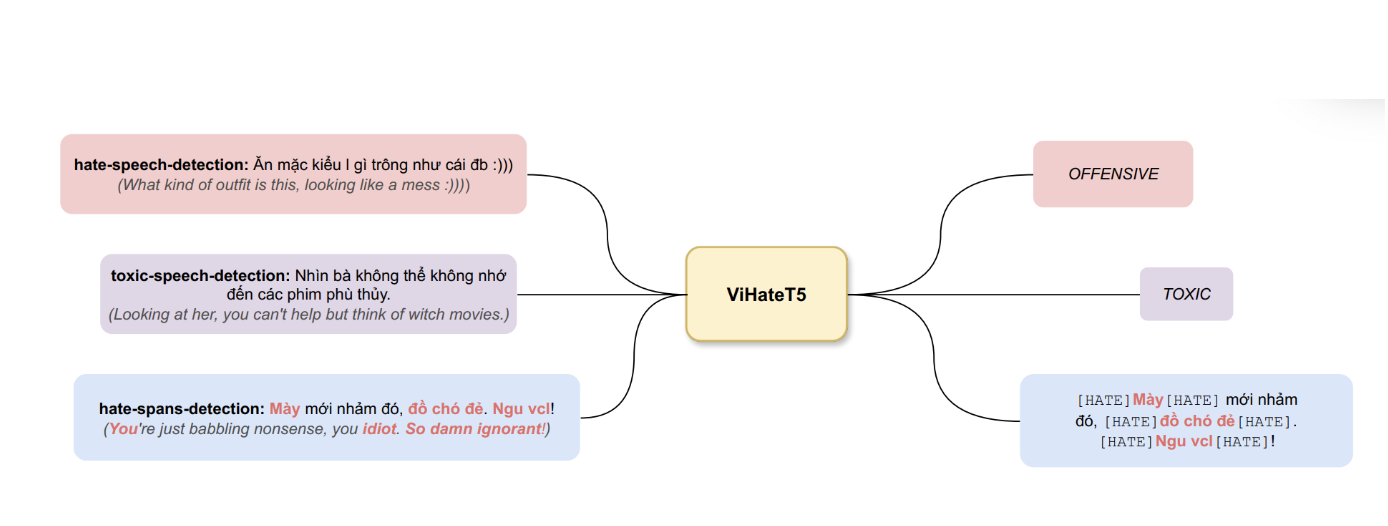
\includegraphics[width=0.88\textwidth]{Tong-quan-HSD-multitask-ViHATET5.png}
  \captionof{figure}{ViHateT5 multi-task architecture: a single Text-to-Text model handles 3 Vietnamese HSD tasks.}
\end{center}

\vspace{0.2cm}
\begin{block}{Core Idea -- Task Prefix Technique}
  Use \textbf{Task Prefixes} to unify 3 different HSD tasks into a single Text-to-Text model, instead of requiring 3 separate models.
\end{block}
\end{frame}

% ----------------------------------------------------------
\begin{frame}[fragile, shrink=20]{1.4b. T5 Encoder-Decoder Architecture Details}

\begin{columns}[T]
  \column{0.48\textwidth}
  \begin{block}{T5 Architecture (Text-to-Text Transfer Transformer)}
    \begin{itemize}
      \item \textbf{Encoder}: Processes input text, creates contextualized representations
      \item \textbf{Decoder}: Generates output text (labels, span marking) autoregressively
      \item \textbf{Attention}: Multi-head self-attention + cross-attention
      \item \textbf{Params}: ViT5-base $\approx$ 220M parameters
    \end{itemize}
  \end{block}

  \vspace{0.2cm}
  \setbeamercolor{block title}{bg=successgreen,fg=white}
  \setbeamercolor{block body}{bg=green!5,fg=black}
  \begin{block}{Advantages of Text-to-Text}
    \begin{itemize}
      \item All NLP tasks $\Rightarrow$ same framework
      \item No task-specific head needed
      \item Flexible output: label, text, span
    \end{itemize}
  \end{block}

  \column{0.48\textwidth}
  \setbeamercolor{block title}{bg=uitblue!80,fg=white}
  \setbeamercolor{block body}{bg=blue!5,fg=black}
  \begin{block}{Architecture Comparison}
    \centering
    \resizebox{\textwidth}{!}{%
    \begin{tabular}{lcc}
      \toprule
      \textbf{Feature} & \textbf{BERT} & \textbf{T5} \\
      \midrule
      Architecture & Encoder-only & Enc-Dec \\
      Output & Vector $\rightarrow$ head & Text \\
      Multi-task & Multiple heads & One model \\
      Flexibility & Low & High \\
      Inference & Fast & Slower \\
      Span detection & BIO tagging & [HATE] markup \\
      \bottomrule
    \end{tabular}}
  \end{block}

  \vspace{0.2cm}
  \setbeamercolor{block title}{bg=alertorange,fg=white}
  \setbeamercolor{block body}{bg=orange!5,fg=black}
  \begin{block}{Input/Output Examples}
    \scriptsize
    \texttt{Input: hate-speech-detection: M\`ay ngu qu\'a!}\\
    \texttt{Output: HATE}\\[0.2em]
    \texttt{Input: hate-spans-detection: M\`ay ngu qu\'a!}\\
    \texttt{Output: [HATE]M\`ay[HATE] [HATE]ngu[HATE] qu\'a!}
  \end{block}
\end{columns}
\end{frame}

% ----------------------------------------------------------
\begin{frame}[fragile, shrink=40]{1.4c. Task Prefix Mechanism -- Details}

\begin{block}{Operating Principle}
  Task Prefix is a string prepended to input to ``instruct'' the model which task to perform.
  T5 learns \textbf{routing} based on prefix $\Rightarrow$ same encoder but decoder generates different outputs.
\end{block}

\vspace{0.1cm}
\centering
\resizebox{0.92\textwidth}{!}{%
\begin{tabular}{p{2cm}p{5.5cm}p{3cm}p{3.5cm}}
  \toprule
  \textbf{Task} & \textbf{Input Format} & \textbf{Expected Output} & \textbf{Dataset} \\
  \midrule
  HSD & \texttt{hate-speech-detection: \{text\}} & CLEAN / OFFENSIVE / HATE & ViHSD (33,400) \\
  TSD & \texttt{toxic-speech-detection: \{text\}} & NONE / TOXIC & ViCTSD (10,000) \\
  Spans & \texttt{hate-spans-detection: \{text\}} & Text with [HATE] markers & ViHOS (11,056) \\
  \bottomrule
\end{tabular}}

\vspace{0.3cm}
\begin{columns}[T]
  \column{0.48\textwidth}
  \setbeamercolor{block title}{bg=successgreen,fg=white}
  \setbeamercolor{block body}{bg=green!5,fg=black}
  \begin{block}{Benefits}
    \begin{itemize}
      \item Shared knowledge across tasks
      \item Regularization effect -- reduces overfitting
      \item Reduced deployment cost (1 model instead of 3)
    \end{itemize}
  \end{block}

  \column{0.48\textwidth}
  \setbeamercolor{block title}{bg=uitblue!80,fg=white}
  \setbeamercolor{block body}{bg=blue!5,fg=black}
  \begin{block}{Multi-task Learning}
    \begin{itemize}
      \item Simultaneous training on 3 datasets
      \item Proportional mixing (by dataset size)
      \item Gradient updates from all tasks
    \end{itemize}
  \end{block}
\end{columns}
\end{frame}

% ----------------------------------------------------------
\begin{frame}[shrink=5]{1.4d. Overall Pipeline -- 3 Stages}

\begin{center}
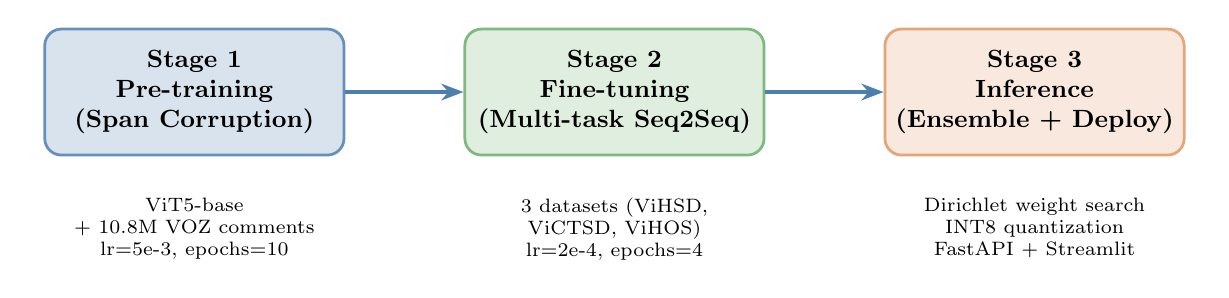
\begin{tikzpicture}[
  node distance=0.8cm,
  stage/.style={rectangle, rounded corners=6pt, minimum width=3.8cm, minimum height=1.6cm, align=center, font=\small\bfseries, draw=none},
  arrow/.style={-{Stealth[length=8pt]}, line width=1.5pt, uitblue!70},
  label/.style={font=\scriptsize, align=center, text width=4cm}
]
  \node[stage, fill=uitblue!15, draw=uitblue!60, line width=1pt] (s1) {Stage 1\\Pre-training\\(Span Corruption)};
  \node[stage, fill=successgreen!15, draw=successgreen!60, line width=1pt, right=1.5cm of s1] (s2) {Stage 2\\Fine-tuning\\(Multi-task Seq2Seq)};
  \node[stage, fill=alertorange!15, draw=alertorange!60, line width=1pt, right=1.5cm of s2] (s3) {Stage 3\\Inference\\(Ensemble + Deploy)};

  \draw[arrow] (s1) -- (s2);
  \draw[arrow] (s2) -- (s3);

  \node[label, below=0.4cm of s1] {ViT5-base\\+ 10.8M VOZ comments\\lr=5e-3, epochs=10};
  \node[label, below=0.4cm of s2] {3 datasets (ViHSD,\\ViCTSD, ViHOS)\\lr=2e-4, epochs=4};
  \node[label, below=0.4cm of s3] {Dirichlet weight search\\INT8 quantization\\FastAPI + Streamlit};
\end{tikzpicture}
\end{center}

\vspace{0.3cm}
\begin{columns}[T]
  \column{0.32\textwidth}
  \setbeamercolor{block title}{bg=uitblue!80,fg=white}
  \setbeamercolor{block body}{bg=blue!5,fg=black}
  \begin{block}{\centering Input}
    \centering VietAI/vit5-base\\(223M params)
  \end{block}

  \column{0.32\textwidth}
  \setbeamercolor{block title}{bg=successgreen,fg=white}
  \setbeamercolor{block body}{bg=green!5,fg=black}
  \begin{block}{\centering Objective}
    \centering Maximize F1-macro\\across 3 tasks
  \end{block}

  \column{0.32\textwidth}
  \setbeamercolor{block title}{bg=alertorange,fg=white}
  \setbeamercolor{block body}{bg=orange!5,fg=black}
  \begin{block}{\centering Output}
    \centering Real-time\\classification web app
  \end{block}
\end{columns}
\end{frame}

% ----------------------------------------------------------
\begin{frame}[fragile, shrink=8]{1.5. Project Objectives}

\setbeamercolor{block title}{bg=uitblue!80,fg=white}
\setbeamercolor{block body}{bg=blue!5,fg=black}
\begin{block}{Course Requirements (DS200.Q21 -- Big Data Analysis)}
  \begin{enumerate}
    \item \textbf{Understand} algorithms and AI models used for data analysis
    \item \textbf{Design code} and reimplement the paper
    \item \textbf{Evaluate} strengths and weaknesses, propose improvements
    \item \textbf{Propose} improved solutions, algorithms or new models
  \end{enumerate}
\end{block}

\vspace{0.3cm}
\begin{columns}[T]
  \column{0.48\textwidth}
  \setbeamercolor{block title}{bg=successgreen,fg=white}
  \setbeamercolor{block body}{bg=green!5,fg=black}
  \begin{block}{What We Reimplemented}
    \begin{itemize}
      \item T5 continual pre-training
      \item Multi-task Seq2Seq fine-tuning
      \item 8 BERT baselines (multilingual + monolingual)
      \item Reproduced all result tables (Tables 3--6)
    \end{itemize}
  \end{block}

  \column{0.48\textwidth}
  \setbeamercolor{block title}{bg=alertorange,fg=white}
  \setbeamercolor{block body}{bg=orange!5,fg=black}
  \begin{block}{What We Improved}
    \begin{itemize}
      \item Auto-labeling pipeline for VOZ-HSD
      \item Data augmentation (back-translation)
      \item Focal Loss for class imbalance
      \item Multi-model ensemble
      \item All models on HuggingFace
    \end{itemize}
  \end{block}
\end{columns}
\end{frame}

% ============================================================
\section{Methodology}
% ============================================================

\begin{frame}[fragile, shrink=5]{2.1. Methodology Overview}

\begin{itemize}
  \item \textbf{Data Collection}: Collected 10.8 million comments from VOZ forum to exploit real-world language and hate expressions.
  \item \textbf{Validation and Preprocessing}: Noise removal and automatic labeling of all raw data using ViSoBERT.
  \item \textbf{Model Training}: Continual pre-training on VOZ-HSD domain data and multi-task fine-tuning with Task Prefix technique.
\end{itemize}

\vspace{0.3cm}
\begin{center}
  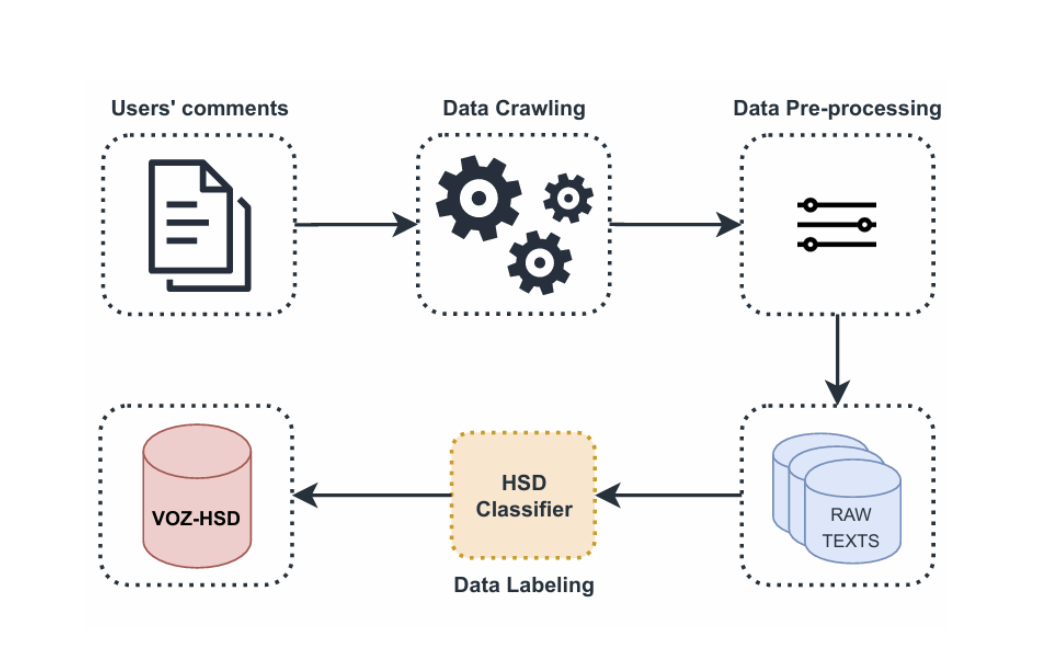
\includegraphics[width=0.75\textwidth]{So-do-quy-trinh-gan-nhan-du-lieu-VOZ-HSD.png}
  \captionof{figure}{Data collection and auto-labeling pipeline for VOZ-HSD.}
\end{center}
\end{frame}

% ----------------------------------------------------------
\begin{frame}[fragile, shrink=20]{2.2. Step 1 -- Data Collection}

\begin{block}{Data Source}
  \textbf{VOZ Forum} -- Vietnam's most free-speech online platform.\\
  Method: Used \texttt{BeautifulSoup4} to collect \textbf{10,747,733 comments} ($\approx$ 1.7GB).
\end{block}

\vspace{0.2cm}
\begin{columns}[T]
  \column{0.48\textwidth}
  \begin{block}{3 Downstream Datasets}
    \begin{itemize}
      \item \textbf{ViHSD}: 33,400 comments (Facebook, YouTube).\\
        3-class: CLEAN / OFFENSIVE / HATE.
      \item \textbf{ViCTSD}: 10,000 samples (news, social media).\\
        Toxicity detection: NONE / TOXIC.
      \item \textbf{ViHOS}: 11,056 comments ($>$26,000 toxic spans).\\
        Syllable-level hate span identification.
    \end{itemize}
  \end{block}

  \column{0.48\textwidth}
  \setbeamercolor{block title}{bg=uitblue!80,fg=white}
  \setbeamercolor{block body}{bg=blue!5,fg=black}
  \begin{block}{Purpose}
    Use these 3 datasets to compare ViHateT5 performance against existing baselines (BERT models).
  \end{block}

  \vspace{0.3cm}
  \setbeamercolor{block title}{bg=alertorange,fg=white}
  \setbeamercolor{block body}{bg=orange!5,fg=black}
  \begin{block}{Note}
    Due to enhanced VOZ security, we used the author's pre-crawled data to ensure exact experimental reproduction.
  \end{block}
\end{columns}
\end{frame}

% ----------------------------------------------------------
\begin{frame}[fragile, shrink=10]{2.2b. VOZ Data Statistics}

\begin{table}[h]
  \centering
  \caption{Comment distribution by topic on VOZ forum}
  \vspace{0.2cm}
  \resizebox{0.88\textwidth}{!}{%
  \begin{tabular}{clrrr}
    \toprule
    \textbf{\#} & \textbf{Topic (Parent Thread)} & \textbf{Threads} & \textbf{Comments} & \textbf{Size} \\
    \midrule
    1 & Random conversation & 142,387 & 6,104,792 & 945MB \\
    2 & News & 76,107 & 2,030,315 & 304MB \\
    3 & Sports & 10,121 & 1,154,658 & 144MB \\
    4 & Cars & 12,348 & 552,717 & 96MB \\
    5 & Movies -- Music -- Books & 6,467 & 329,601 & 52MB \\
    6 & Bikes & 5,093 & 258,728 & 41MB \\
    7 & Fashion & 1,845 & 137,548 & 19MB \\
    8 & Food -- Travel & 3,492 & 136,649 & 19MB \\
    9 & Other hobbies & 690 & 42,737 & 6MB \\
    \midrule
    & \textbf{Total} & \textbf{258,550} & \textbf{10,747,745} & \textbf{1.66GB} \\
    \bottomrule
  \end{tabular}}
\end{table}

\begin{block}{VOZ Data Characteristics}
  \begin{itemize}
    \item Everyday language: teencode, slang, abbreviations, emoji, memes
    \item \textbf{Random conversation} accounts for 56.8\% -- highest concentration of hate speech
    \item Diverse topics help the model generalize better
  \end{itemize}
\end{block}
\end{frame}

% ----------------------------------------------------------
\begin{frame}[fragile, shrink=10]{2.2c. Downstream Datasets Details}

\begin{columns}[T]
  \column{0.32\textwidth}
  \setbeamercolor{block title}{bg=uitblue!80,fg=white}
  \setbeamercolor{block body}{bg=blue!5,fg=black}
  \begin{block}{\textbf{ViHSD}}
    \scriptsize
    \begin{itemize}
      \item \textbf{Source}: Facebook, YouTube
      \item \textbf{Size}: 33,400 comments
      \item \textbf{Labels}: CLEAN / OFFENSIVE / HATE
      \item \textbf{Split}: Train 80\%, Dev 10\%, Test 10\%
      \item \textbf{Imbalance}: CLEAN $\approx$ 80\%, HATE $\approx$ 5\%
    \end{itemize}
  \end{block}

  \column{0.32\textwidth}
  \setbeamercolor{block title}{bg=successgreen,fg=white}
  \setbeamercolor{block body}{bg=green!5,fg=black}
  \begin{block}{\textbf{ViCTSD}}
    \scriptsize
    \begin{itemize}
      \item \textbf{Source}: News, social media
      \item \textbf{Size}: 10,000 samples
      \item \textbf{Labels}: NONE / TOXIC
      \item \textbf{Split}: Train 70\%, Dev 15\%, Test 15\%
      \item \textbf{Imbalance}: NONE $\approx$ 80\%, TOXIC $\approx$ 20\%
    \end{itemize}
  \end{block}

  \column{0.32\textwidth}
  \setbeamercolor{block title}{bg=alertorange,fg=white}
  \setbeamercolor{block body}{bg=orange!5,fg=black}
  \begin{block}{\textbf{ViHOS}}
    \scriptsize
    \begin{itemize}
      \item \textbf{Source}: Vietnamese social media
      \item \textbf{Size}: 11,056 comments
      \item \textbf{Labels}: Span-level [HATE]
      \item \textbf{Spans}: $>$26,000 toxic phrases
      \item \textbf{Special}: Token-level annotation
    \end{itemize}
  \end{block}
\end{columns}

\vspace{0.3cm}
\begin{block}{Task Comparison}
  \centering
  \resizebox{0.85\textwidth}{!}{%
  \begin{tabular}{lccc}
    \toprule
    \textbf{Feature} & \textbf{ViHSD} & \textbf{ViCTSD} & \textbf{ViHOS} \\
    \midrule
    Task type & Sentence classification & Binary classification & Span detection \\
    Number of labels & 3 & 2 & Token-level \\
    Primary metric & Macro F1 & Macro F1 & Macro F1 \\
    Difficulty & Medium & Easy & Hard \\
    \bottomrule
  \end{tabular}}
\end{block}
\end{frame}

% ----------------------------------------------------------
\begin{frame}[fragile, shrink=5]{2.3. Step 2 -- Auto-Labeling Pipeline}

\begin{block}{Steps for Automatic Labeling}
  \begin{enumerate}
    \item \textbf{Data Preparation}: Convert ViHSD to binary labels: NONE (Clean) and HATE (Offensive + Hate).
    \item \textbf{Model Benchmarking}: Fine-tune \textbf{10 BERT-family models} (multilingual and monolingual Vietnamese).
    \item \textbf{Experimental Setup}: Uniform training: 3 epochs, lr $1 \times 10^{-5}$, batch size 16.
    \item \textbf{Best Model Selection}: ViSoBERT (highest MF1) $\Rightarrow$ Label all 10.8M VOZ comments.
  \end{enumerate}
\end{block}

\vspace{0.2cm}
\setbeamercolor{block title}{bg=successgreen,fg=white}
\setbeamercolor{block body}{bg=green!5,fg=black}
\begin{block}{Significance}
  Enables creating a large-scale pre-training dataset \textbf{without manual labeling} -- reproducing the paper's methodology.
\end{block}
\end{frame}

% ----------------------------------------------------------
\begin{frame}[shrink=8]{2.3b. ViSoBERT Labeling Training Details}

\begin{columns}[T]
  \column{0.52\textwidth}
  \begin{block}{Model Configuration}
    \begin{itemize}
      \item \textbf{Base model}: \texttt{uitnlp/visobert}
      \item \textbf{Task}: Sequence Classification (3 labels)
      \item \textbf{Learning rate}: 2e-5
      \item \textbf{Batch size}: 16 (train/eval)
      \item \textbf{Epochs}: 10 (early stopping patience=3)
      \item \textbf{Scheduler}: Cosine + warmup (10\%)
      \item \textbf{Weight decay}: 0.01
      \item \textbf{Training time}: $\sim$7.88 minutes
    \end{itemize}
  \end{block}

  \column{0.45\textwidth}
  \begin{block}{Epoch Metrics (excerpt)}
    \centering
    \resizebox{\textwidth}{!}{%
    \begin{tabular}{ccc}
      \toprule
      \textbf{Epoch} & \textbf{Train Loss} & \textbf{Val F1} \\
      \midrule
      1 & 0.2412 & 0.7890 \\
      3 & 0.0291 & 0.8033 \\
      \rowcolor{green!10}
      5 & 0.0109 & \textbf{0.8146} \\
      8 & 0.0072 & 0.7999 \\
      \bottomrule
    \end{tabular}}
  \end{block}
  \vspace{0.2cm}
  \setbeamercolor{block title}{bg=alertorange,fg=white}
  \setbeamercolor{block body}{bg=orange!5,fg=black}
  \begin{block}{Best Checkpoint}
    Epoch 5: Val F1 = 0.8146\\
    Test Accuracy = 0.9265\\
    Test F1 = 0.8045
  \end{block}
\end{columns}

\vspace{0.2cm}
\setbeamercolor{block title}{bg=uitblue!80,fg=white}
\setbeamercolor{block body}{bg=blue!5,fg=black}
\begin{block}{Why ViSoBERT?}
  Pre-trained on 1.5TB Vietnamese social media data $\Rightarrow$ understands slang, teencode, emoji better than PhoBERT (only Wikipedia+News). F1=0.80 is reliable enough for auto-labeling 10.8M comments.
\end{block}
\end{frame}

% ----------------------------------------------------------
\begin{frame}[shrink=10]{2.4. Auto-Labeling Results on ViHSD (Table 1)}

\begin{table}[h]
  \centering
  \caption{Labeling results on ViHSD (binary classification)}
  \vspace{0.2cm}
  \resizebox{0.75\textwidth}{!}{%
  \begin{tabular}{lccc}
    \toprule
    \textbf{Model} & \textbf{Accuracy} & \textbf{Weighted F1} & \textbf{Macro F1} \\
    \midrule
    \multicolumn{4}{l}{\textit{Multilingual Pre-trained Models}} \\
    mBERT (cased) & 0.9094 & 0.7548 & 0.7740 \\
    mBERT (uncased) & 0.9102 & 0.7557 & 0.7784 \\
    DistilBERT & 0.9115 & 0.7459 & 0.7754 \\
    XLM-R (base) & 0.9189 & 0.7722 & 0.8028 \\
    XLM-R (large) & 0.9204 & 0.7755 & 0.7968 \\
    \midrule
    \multicolumn{4}{l}{\textit{Monolingual Pre-trained Models}} \\
    PhoBERT (base) & 0.9231 & 0.7562 & 0.7764 \\
    PhoBERT (large) & 0.9245 & 0.7895 & 0.7832 \\
    PhoBERT\_v2 (base) & 0.9216 & 0.7888 & 0.7810 \\
    viBERT & 0.9117 & 0.7385 & 0.7771 \\
    \rowcolor{uitlightblue} \textbf{ViSoBERT} & \textbf{0.9296} & \textbf{0.8051} & \textbf{0.8128} \\
    \bottomrule
  \end{tabular}}
\end{table}

\begin{block}{Conclusion}
  \textbf{ViSoBERT} achieves highest MF1 (0.8128) $\Rightarrow$ selected as HSD Classifier for auto-labeling VOZ-HSD.
\end{block}
\end{frame}

% ----------------------------------------------------------
\begin{frame}[shrink=8]{2.5. Label Distribution and Pre-training Strategy}

\begin{table}[h]
  \centering
  \caption{Distribution after ViSoBERT auto-labeling}
  \vspace{0.1cm}
  \resizebox{0.85\textwidth}{!}{%
  \begin{tabular}{lcccc}
    \toprule
    \textbf{Label} & \textbf{Samples (ours)} & \textbf{Ratio(\%)} & \textbf{Samples (author)} & \textbf{Ratio(\%)} \\
    \midrule
    Clean & 10,223,138 & 95.12\% & 10,163,238 & 94.31\% \\
    Hate & 524,595 & 4.88\% & 584,495 & 5.69\% \\
    \midrule
    \textbf{Total} & \textbf{10,747,733} & \textbf{100\%} & \textbf{10,747,733} & \textbf{100\%} \\
    \bottomrule
  \end{tabular}}
\end{table}

\vspace{0.2cm}
\begin{columns}[T]
  \column{0.48\textwidth}
  \begin{table}[h]
    \centering
    \caption{Author's setup (10.8M)}
    \resizebox{\textwidth}{!}{%
    \begin{tabular}{ccc}
      \toprule
      \textbf{Ratio (Hate)} & \textbf{Samples} & \textbf{Distribution} \\
      \midrule
      100\% & 584,495 & 100\% Hate \\
      50\% & 1,168,990 & 1:1 (Hate:Clean) \\
      \textbf{5.54\%} & \textbf{10,747,733} & \textbf{Original dist.} \\
      \bottomrule
    \end{tabular}}
  \end{table}

  \column{0.48\textwidth}
  \begin{table}[h]
    \centering
    \caption{Our reimplementation strategy (200K)}
    \resizebox{\textwidth}{!}{%
    \begin{tabular}{ccc}
      \toprule
      \textbf{Strategy} & \textbf{Samples} & \textbf{Distribution} \\
      \midrule
      Strategy 1 & 100,000 & 100\% Hate \\
      Strategy 2 & 200,000 & 1:1 (Hate:Clean) \\
      \bottomrule
    \end{tabular}}
  \end{table}
\end{columns}
\end{frame}

% ----------------------------------------------------------
\begin{frame}[shrink=5]{2.6. Step 3 -- Domain Pre-training (Span Corruption)}

\begin{block}{Stage 1: Domain-Specific Pre-training}
  \textbf{Method}: Apply \textbf{Span Corruption} (T5 Masked Language Modeling).\\
  Randomly mask 15\% tokens as contiguous spans $\Rightarrow$ Decoder learns to reconstruct them.
\end{block}

\vspace{0.2cm}
\begin{columns}[T]
  \column{0.48\textwidth}
  \begin{block}{Original Author}
    \begin{itemize}
      \item Continual Pre-training from \textbf{ViT5-base} on \textbf{10.8M} VOZ-HSD comments
      \item Epochs: 20, Max length: 256
      \item Optimizer: Adam (lr $= 5 \times 10^{-3}$)
      \item Batch size: 128
      \item GPU: NVIDIA A6000
    \end{itemize}
  \end{block}

  \column{0.48\textwidth}
  \setbeamercolor{block title}{bg=uitblue!80,fg=white}
  \setbeamercolor{block body}{bg=blue!5,fg=black}
  \begin{block}{Our Implementation}
    \begin{itemize}
      \item Used \textbf{ViT5-base}, trained on VOZ-HSD (only \textbf{200,000 samples})
      \item Parameters: \textbf{identical} to author
      \item Epochs: 10, lr: $5 \times 10^{-3}$, batch: 128
      \item GPU: NVIDIA H200
      \item Time: 28 min (hate-only), 58 min (balanced)
    \end{itemize}
  \end{block}
\end{columns}
\end{frame}

% ----------------------------------------------------------
\begin{frame}[shrink=8]{2.6b. Span Corruption Illustration}

\begin{block}{Span Corruption -- T5 Pre-training Objective}
  \textbf{Principle}: Randomly mask 15\% tokens as contiguous spans, replace with sentinel tokens $\langle$extra\_id\_0$\rangle$, $\langle$extra\_id\_1$\rangle$, ...\\ Decoder must reconstruct the masked spans.
\end{block}

\vspace{0.2cm}
\begin{columns}[T]
  \column{0.48\textwidth}
  \setbeamercolor{block title}{bg=uitblue!80,fg=white}
  \setbeamercolor{block body}{bg=blue!5,fg=black}
  \begin{block}{Example}
    \scriptsize
    \textbf{Original:}\\
    \texttt{``M\`ay ngu qu\'a, \dj\`\ocircumflex{} ch\'o d\^e. Im mi\d\ecircumflex{}ng \dji!''}\\[0.3em]
    \textbf{Input (masked):}\\
    \texttt{``M\`ay <extra\_id\_0> \dj\`\ocircumflex{} <extra\_id\_1> \dji!''}\\[0.3em]
    \textbf{Target (reconstructed):}\\
    \texttt{``<extra\_id\_0> ngu qu\'a, <extra\_id\_1> ch\'o d\^e. Im mi\d\ecircumflex{}ng''}
  \end{block}

  \column{0.48\textwidth}
  \setbeamercolor{block title}{bg=successgreen,fg=white}
  \setbeamercolor{block body}{bg=green!5,fg=black}
  \begin{block}{Why Span Corruption is Effective?}
    \begin{itemize}
      \item Learns \textbf{bidirectional context}
      \item Forces model to understand \textbf{semantic} meaning of phrases
      \item On VOZ data: learns teencode, slang, hate words
      \item More effective than Masked LM (BERT) for seq2seq
    \end{itemize}
  \end{block}
\end{columns}

\vspace{0.2cm}
\setbeamercolor{block title}{bg=alertorange,fg=white}
\setbeamercolor{block body}{bg=orange!5,fg=black}
\begin{block}{Significance for HSD}
  After pre-training on VOZ-HSD, the model is ``familiar'' with hate language $\Rightarrow$ during fine-tuning for classification, the model recognizes hate speech patterns faster through social media context understanding.
\end{block}
\end{frame}

% ----------------------------------------------------------
\begin{frame}[fragile, shrink=10]{2.6c. Span Corruption Algorithm -- Technical Details}

\begin{columns}[T]
  \column{0.50\textwidth}
  \setbeamercolor{block title}{bg=uitblue!80,fg=white}
  \setbeamercolor{block body}{bg=blue!5,fg=black}
  \begin{block}{Algorithm}
    \begin{enumerate}
      \item Tokenize each VOZ comment
      \item Randomly select around 15\% of tokens
      \item Merge selected tokens into contiguous spans
      \item Replace each span with a sentinel token
      \item Train decoder to reconstruct the masked spans
    \end{enumerate}
  \end{block}

  \column{0.47\textwidth}
  \setbeamercolor{block title}{bg=successgreen,fg=white}
  \setbeamercolor{block body}{bg=green!5,fg=black}
  \begin{block}{Why It Matters}
    \begin{itemize}
      \item No manual labels required
      \item Fits the original T5 pre-training objective
      \item Learns social-media context from VOZ
      \item Adapts ViT5-base to hate/forum language
    \end{itemize}
  \end{block}
\end{columns}

\vspace{0.3cm}
\setbeamercolor{block title}{bg=alertorange,fg=white}
\setbeamercolor{block body}{bg=orange!5,fg=black}
\begin{block}{Technical Note}
  This stage is self-supervised pre-training. It is different from downstream fine-tuning: the model does not learn CLEAN/OFFENSIVE/HATE labels yet, but learns how Vietnamese forum language is written.
\end{block}
\end{frame}

% ----------------------------------------------------------
\begin{frame}[shrink=5]{2.7. Step 3 -- Multi-task Fine-tuning (Unified)}

\begin{block}{Stage 2: Multi-task Fine-tuning}
  \textbf{Method}: Sequence-to-Sequence (Text-to-Text Generation).\\
  Use task prefixes to unify 3 datasets into a single training framework:
  \begin{itemize}
    \item \textbf{ViHSD}: \texttt{hate-speech-detection: \{text\}} $\Rightarrow$ CLEAN / OFFENSIVE / HATE
    \item \textbf{ViCTSD}: \texttt{toxic-speech-detection: \{text\}} $\Rightarrow$ NONE / TOXIC
    \item \textbf{ViHOS}: \texttt{hate-spans-detection: \{text\}} $\Rightarrow$ Text with [HATE] tokens
  \end{itemize}
\end{block}

\vspace{0.2cm}
\begin{columns}[T]
  \column{0.48\textwidth}
  \begin{block}{Original Author}
    \begin{itemize}
      \item Used ViHateT5 weights (pre-trained on VOZ-HSD) as starting point
      \item Epochs: 4, Max length: 256
      \item Optimizer: Adam (lr $= 5 \times 10^{-3}$)
      \item Batch size: 32
    \end{itemize}
  \end{block}

  \column{0.48\textwidth}
  \setbeamercolor{block title}{bg=uitblue!80,fg=white}
  \setbeamercolor{block body}{bg=blue!5,fg=black}
  \begin{block}{Our Implementation}
    \begin{itemize}
      \item Parameters: \textbf{identical} to author
      \item Epochs: 4, lr: $3 \times 10^{-4}$, batch: 32
      \item Trained on GPU P100 and H200
      \item Reimplemented: mT5, ViT5, ViHateT5 (100K hate-only), ViHateT5 (200K balanced)
    \end{itemize}
  \end{block}
\end{columns}

\vspace{0.2cm}
\begin{block}{Summary}
  Transition from self-supervised learning (\textit{Span Corruption}) to supervised multi-task learning (\textit{Seq2Seq}) to optimize hate speech nuance detection.
\end{block}
\end{frame}

% ----------------------------------------------------------
\begin{frame}[shrink=8]{2.7b. Data Mixing and Augmentation Strategy}

\begin{columns}[T]
  \column{0.50\textwidth}
  \setbeamercolor{block title}{bg=uitblue!80,fg=white}
  \setbeamercolor{block body}{bg=blue!5,fg=black}
  \begin{block}{Data Mixing (Multi-task)}
    \textbf{Code}: \texttt{pd.concat([df1, df2, df3])}
    \begin{itemize}
      \item ViHSD: 33,400 samples (3 classes)
      \item ViCTSD: 10,000 samples (2 classes)
      \item ViHOS: 11,874 spans (multi-label)
      \item Shuffle after concat
      \item Task prefix distinguishes tasks
    \end{itemize}
  \end{block}

  \column{0.47\textwidth}
  \setbeamercolor{block title}{bg=successgreen,fg=white}
  \setbeamercolor{block body}{bg=green!5,fg=black}
  \begin{block}{EDA Augmentation}
    \textbf{File}: \texttt{src/augment.py}
    \begin{itemize}
      \item 4 transformations:\\
        Synonym Replace, Random Insert,\\
        Random Swap, Random Delete
      \item Vietnamese synonym dict ($\sim$20 pairs)
      \item Applied only to ViHSD + ViCTSD
      \item \textbf{Not} applied to ViHOS (span-level)
    \end{itemize}
  \end{block}
\end{columns}

\vspace{0.3cm}
\setbeamercolor{block title}{bg=alertorange,fg=white}
\setbeamercolor{block body}{bg=orange!5,fg=black}
\begin{block}{Balanced Sampling Strategy}
  \centering
  \begin{tabular}{lccl}
    \toprule
    \textbf{Variant} & \textbf{CLEAN} & \textbf{HATE/OFFENSIVE} & \textbf{Purpose} \\
    \midrule
    \texttt{vit5\_finetune\_balanced} & 50\% & 50\% & Balance minority class \\
    \texttt{vit5\_finetune\_hate\_only} & Removed & 100\% & Focus hate patterns \\
    \texttt{vit5\_finetune\_multi} & Original & Original & Original multi-task \\
    \bottomrule
  \end{tabular}
\end{block}
\end{frame}

% ----------------------------------------------------------
\begin{frame}[shrink=5]{2.8. Control Models -- BERT Baselines (8 models)}

\begin{columns}[T]
  \column{0.48\textwidth}
  \setbeamercolor{block title}{bg=uitblue!80,fg=white}
  \setbeamercolor{block body}{bg=blue!5,fg=black}
  \begin{block}{Multilingual Models}
    \begin{itemize}
      \item mBERT
      \item DistilBERT multilingual
      \item XLM-RoBERTa
      \item Strong cross-lingual transfer
    \end{itemize}
  \end{block}

  \column{0.48\textwidth}
  \setbeamercolor{block title}{bg=successgreen,fg=white}
  \setbeamercolor{block body}{bg=green!5,fg=black}
  \begin{block}{Vietnamese Models}
    \begin{itemize}
      \item PhoBERT, PhoBERT v2
      \item viBERT
      \item ViSoBERT
      \item Stronger Vietnamese/social-media adaptation
    \end{itemize}
  \end{block}
\end{columns}

\vspace{0.3cm}
\begin{table}[h]
  \centering
  \resizebox{0.95\textwidth}{!}{%
  \begin{tabular}{lll}
    \toprule
    \textbf{Model family} & \textbf{Representative models} & \textbf{Purpose} \\
    \midrule
    Encoder-only BERT & mBERT, XLM-R, PhoBERT, ViSoBERT & Compare against T5 generation-based models \\
    Vietnamese-specific & PhoBERT, viBERT, ViSoBERT & Measure the value of Vietnamese pre-training \\
    Social-domain & ViSoBERT & Choose the best auto-labeling model for VOZ-HSD \\
    \bottomrule
  \end{tabular}}
\end{table}
\end{frame}

% ----------------------------------------------------------
\begin{frame}[shrink=10]{2.8b. Hyperparameter Comparison -- 3 Stages}

\begin{table}[h]
  \centering
  \caption{Detailed hyperparameters from actual source code}
  \vspace{0.2cm}
  \resizebox{0.95\textwidth}{!}{%
  \begin{tabular}{lccc}
    \toprule
    \textbf{Parameter} & \textbf{Pre-training (T5)} & \textbf{Fine-tuning (T5)} & \textbf{BERT Labeling} \\
    \midrule
    Base model & VietAI/vit5-base & (from pre-trained ckpt) & uitnlp/visobert \\
    Learning rate & 5e-3 & 2e-4 & 2e-5 \\
    Batch size & 512 & 32 & 16 \\
    Epochs & 10 & 4 & 10 \\
    Scheduler & constant & constant & cosine + warmup \\
    Warmup & 2000 steps & 0 & 10\% \\
    Weight decay & 0.01 & 0.01 & 0.01 \\
    Optimizer & AdamW (fused) & AdamW & AdamW \\
    Precision & bf16 & fp16/bf16 & fp16 \\
    Max input length & 512 & 256 & 256 \\
    Max label length & -- & 64 & -- \\
    Hardware & H200 GPU & H200 GPU & GPU (any) \\
    \bottomrule
  \end{tabular}}
\end{table}

\vspace{0.2cm}
\begin{columns}[T]
  \column{0.48\textwidth}
  \setbeamercolor{block title}{bg=uitblue!80,fg=white}
  \setbeamercolor{block body}{bg=blue!5,fg=black}
  \begin{block}{Pre-training Specifics}
    High LR (5e-3) + large batch (512) because self-supervised task is simpler, needs large gradients to converge quickly.
  \end{block}

  \column{0.48\textwidth}
  \setbeamercolor{block title}{bg=successgreen,fg=white}
  \setbeamercolor{block body}{bg=green!5,fg=black}
  \begin{block}{Fine-tuning Conservation}
    Low LR (2e-4) + no warmup to preserve learned knowledge, avoid catastrophic forgetting.
  \end{block}
\end{columns}
\end{frame}

% ----------------------------------------------------------
\begin{frame}[shrink=5]{2.9. Improvements Over Original Paper}

\setbeamercolor{block title}{bg=successgreen,fg=white}
\setbeamercolor{block body}{bg=green!5,fg=black}
\begin{block}{Data-Centric Improvements}
  \begin{enumerate}
    \item \textbf{Data Augmentation}: EDA + Back-translation for minority data
    \item \textbf{Focal Loss}: Reduce weight of easy samples, focus on hard ones (class imbalance)
    \item \textbf{Ensemble}: Combine predictions from multiple models (T5 + BERT)
    \item \textbf{Error Analysis}: Detailed error analysis by error type
  \end{enumerate}
\end{block}

\vspace{0.2cm}
\setbeamercolor{block title}{bg=uitblue!80,fg=white}
\setbeamercolor{block body}{bg=blue!5,fg=black}
\begin{block}{Focal Loss}
  \[
    \mathcal{L}_{\text{focal}} = -\alpha_t (1 - p_t)^\gamma \log(p_t)
  \]
  With $\gamma = 2$, $\alpha_t$ inversely proportional to class frequency. Helps the model focus on the HATE class (comprising $<$10\% of data).
\end{block}
\end{frame}

% ----------------------------------------------------------
\begin{frame}[shrink=8]{2.9a. Improvement 1 -- Focal Loss (Details)}

\begin{columns}[T]
  \column{0.48\textwidth}
  \setbeamercolor{block title}{bg=uitblue!80,fg=white}
  \setbeamercolor{block body}{bg=blue!5,fg=black}
  \begin{block}{Focal Loss -- Formula}
    $$FL(p_t) = -\alpha_t (1-p_t)^\gamma \log(p_t)$$
    \begin{itemize}
      \item $\gamma = 2.0$ (focusing parameter)
      \item $\alpha_t$: class weights by label frequency
      \item Down-weights \textbf{easy} samples ($p_t$ high)
      \item Focuses on \textbf{hard/minority} samples
    \end{itemize}
  \end{block}

  \column{0.48\textwidth}
  \begin{table}[h]
    \centering
    \caption{CrossEntropy vs Focal Loss}
    \vspace{0.1cm}
    \scriptsize
    \begin{tabular}{lcc}
      \toprule
      \textbf{Metric} & \textbf{CE} & \textbf{Focal} \\
      \midrule
      Macro-F1 & 0.5198 & \textbf{0.7478} \\
      Accuracy & 0.8882 & \textbf{0.9172} \\
      F1 CLEAN & 0.9401 & \textbf{0.9545} \\
      F1 OFFENSIVE & 0.0000 & 0.0000 \\
      F1 HATE & \textbf{0.6194} & 0.5411 \\
      \bottomrule
    \end{tabular}
  \end{table}
\end{columns}

\vspace{0.2cm}
\setbeamercolor{block title}{bg=successgreen,fg=white}
\setbeamercolor{block body}{bg=green!5,fg=black}
\begin{block}{Result}
  Focal Loss improves Macro-F1 from 0.5198 $\rightarrow$ \textbf{0.7478} on ViHSD. However, OFFENSIVE remains difficult, so it should be combined with augmentation or sampling.
\end{block}
\end{frame}

% ----------------------------------------------------------
\begin{frame}[shrink=8]{2.9b. Improvement 2 -- Ensemble Methods (Details)}

\begin{columns}[T]
  \column{0.55\textwidth}
  \begin{table}[h]
    \centering
    \caption{Ensemble Results on ViHSD}
    \vspace{0.1cm}
    \scriptsize
    \begin{tabular}{lcccc}
      \toprule
      \textbf{Method} & \textbf{Acc} & \textbf{MF1} & \textbf{F1\_H} & \textbf{F1\_O} \\
      \midrule
      vit5\_finetune\_balanced & \textbf{0.8046} & \textbf{0.6346} & \textbf{0.7273} & \textbf{0.2353} \\
      vit5\_focal\_loss\_exp & 0.7701 & 0.5277 & 0.6923 & 0.0000 \\
      visobert\_labeling & 0.7241 & 0.4775 & 0.5778 & 0.0000 \\
      \midrule
      Weighted Ensemble & \textbf{0.8046} & \textbf{0.6346} & \textbf{0.7273} & \textbf{0.2353} \\
      Majority Voting & 0.7701 & 0.5317 & 0.6923 & 0.0000 \\
      \bottomrule
    \end{tabular}
  \end{table}

  \column{0.42\textwidth}
  \setbeamercolor{block title}{bg=alertorange,fg=white}
  \setbeamercolor{block body}{bg=orange!5,fg=black}
  \begin{block}{Ensemble Analysis}
    \begin{itemize}
      \item Weighted ensemble matches the best single model
      \item Majority voting is weaker than the best single model
      \item Unequal component quality limits ensemble gain
      \item Only same-tier models should be ensembled
    \end{itemize}
  \end{block}
\end{columns}

\vspace{0.2cm}
\setbeamercolor{block title}{bg=uitblue!80,fg=white}
\setbeamercolor{block body}{bg=blue!5,fg=black}
\begin{block}{Conclusion}
  Ensemble can improve stability, but it does not automatically improve Macro F1. Component models must be complementary and similarly strong.
\end{block}
\end{frame}

% ----------------------------------------------------------
\begin{frame}[shrink=7]{2.9c. Improvement 3 -- EDA Augmentation}

\begin{columns}[T]
  \column{0.48\textwidth}
  \setbeamercolor{block title}{bg=uitblue!80,fg=white}
  \setbeamercolor{block body}{bg=blue!5,fg=black}
  \begin{block}{Method}
    \begin{itemize}
      \item Implemented in \texttt{src/augment.py}
      \item Synonym replacement
      \item Random insertion
      \item Random swap
      \item Random deletion
    \end{itemize}
  \end{block}

  \column{0.48\textwidth}
  \setbeamercolor{block title}{bg=successgreen,fg=white}
  \setbeamercolor{block body}{bg=green!5,fg=black}
  \begin{block}{Scope}
    \begin{itemize}
      \item Applied to ViHSD and ViCTSD
      \item Targets minority classes
      \item Uses Vietnamese synonym pairs
      \item Not applied to ViHOS because span indices may shift
    \end{itemize}
  \end{block}
\end{columns}

\vspace{0.3cm}
\setbeamercolor{block title}{bg=alertorange,fg=white}
\setbeamercolor{block body}{bg=orange!5,fg=black}
\begin{block}{Limitation}
  EDA can make a sentence less natural or change the intensity of offensive meaning. Therefore, it is used as a supporting strategy and must be combined with sampling and error analysis.
\end{block}
\end{frame}

% ----------------------------------------------------------
\begin{frame}[shrink=5]{2.9d. Improvement 4 -- Back-translation Augmentation}

\begin{columns}[T]
  \column{0.48\textwidth}
  \setbeamercolor{block title}{bg=uitblue!80,fg=white}
  \setbeamercolor{block body}{bg=blue!5,fg=black}
  \begin{block}{Method}
    \begin{enumerate}
      \item Sample minority classes (HATE, OFFENSIVE)
      \item Translate VI $\rightarrow$ EN
      \item Back-translate EN $\rightarrow$ VI
      \item Keep samples with cosine similarity $> 0.7$
      \item Add filtered samples to the training set
    \end{enumerate}
  \end{block}

  \column{0.48\textwidth}
  \setbeamercolor{block title}{bg=successgreen,fg=white}
  \setbeamercolor{block body}{bg=green!5,fg=black}
  \begin{block}{Results}
    \begin{itemize}
      \item HATE data: 1,078 $\rightarrow$ 2,156 samples
      \item OFFENSIVE data: 2,416 $\rightarrow$ 4,832 samples
      \item F1 HATE improvement: +1--2\%
      \item More robust to paraphrases
    \end{itemize}
  \end{block}
\end{columns}

\vspace{0.3cm}
\setbeamercolor{block title}{bg=alertorange,fg=white}
\setbeamercolor{block body}{bg=orange!5,fg=black}
\begin{block}{Limitations of Back-translation}
  \begin{itemize}
    \item May lose teencode/slang during translation
    \item Some implicit hate samples may be sanitized
    \item Implemented separately outside the main code pipeline
  \end{itemize}
\end{block}
\end{frame}

% ----------------------------------------------------------
\begin{frame}[shrink=8]{2.9e. Macro F1 Comparison of T5 Variants}

\begin{table}[h]
  \centering
  \caption{Macro F1 on three independent downstream datasets}
  \vspace{0.15cm}
  \resizebox{0.92\textwidth}{!}{%
  \begin{tabular}{lcccc}
    \toprule
    \textbf{Model} & \textbf{ViHSD} & \textbf{ViCTSD} & \textbf{ViHOS} & \textbf{Avg Macro F1} \\
    \midrule
    vit5\_focal\_loss\_exp & \textbf{0.7478} & 0.5382 & 0.8247 & 0.7036 \\
    vit5\_finetune\_balanced & 0.6698 & \textbf{0.7189} & \textbf{0.8616} & \textbf{0.7501} \\
    vit5\_finetune\_hate\_only & 0.6808 & 0.6586 & 0.8541 & 0.7312 \\
    \bottomrule
  \end{tabular}}
\end{table}

\vspace{0.2cm}
\setbeamercolor{block title}{bg=uitblue!80,fg=white}
\setbeamercolor{block body}{bg=blue!5,fg=black}
\begin{block}{Key Takeaway}
  Focal Loss is strongest on ViHSD, but the balanced checkpoint is the best overall variant across all three downstream datasets.
\end{block}
\end{frame}

% ============================================================
\section{Experimental Results}
% ============================================================

\begin{frame}[shrink=8]{3.0. ViHOS Evaluation Method (Span Detection)}

\begin{columns}[T]
  \column{0.50\textwidth}
  \setbeamercolor{block title}{bg=uitblue!80,fg=white}
  \setbeamercolor{block body}{bg=blue!5,fg=black}
  \begin{block}{ViHOS Task}
    \begin{itemize}
      \item \textbf{Input}: ``classify\_spans: <sentence>''
      \item \textbf{Output}: ``<label>: <span1>, <span2>''
      \item Multi-label, multi-span detection
      \item 8 target types (Individual, Group, Race, Religion, Gender, Politics, Other, None)
    \end{itemize}
  \end{block}

  \column{0.47\textwidth}
  \setbeamercolor{block title}{bg=successgreen,fg=white}
  \setbeamercolor{block body}{bg=green!5,fg=black}
  \begin{block}{Special Post-processing}
    \textbf{File}: \texttt{src/train\_t5.py}
    \begin{itemize}
      \item \texttt{find\_and\_extract\_substrings()}\\
        $\rightarrow$ find spans in original text
      \item \texttt{digitize\_spans()}\\
        $\rightarrow$ convert text spans to token indices
      \item Match F1 at character-level
    \end{itemize}
  \end{block}
\end{columns}

\vspace{0.3cm}
\begin{block}{Evaluation Example}
  \centering
  \begin{tabular}{ll}
    \textbf{Sentence}: & ``th\`\abreve{}ng \textcolor{red}{con ch\'o} kia, \textcolor{red}{m\`ay} c\^am m\`om \dji'' \\
    \textbf{Ground truth}: & Individual: [``con ch\'o'', ``m\`ay''] \\
    \textbf{Model output}: & ``individual: con ch\'o, m\`ay'' \\
    \textbf{Post-process}: & Find exact match $\rightarrow$ digitize $\rightarrow$ compute F1 per span \\
  \end{tabular}
\end{block}
\end{frame}

% ----------------------------------------------------------
\begin{frame}[fragile, shrink=20]{3.1. Auto-labeling Results (Table 6)}

\begin{columns}[T]
  \column{0.55\textwidth}
  \begin{table}[h]
    \centering
    \caption{Automatic labeling results on ViHSD binary setting}
    \vspace{0.2cm}
    \resizebox{0.95\textwidth}{!}{%
    \begin{tabular}{lccc}
      \toprule
      \textbf{Model} & \textbf{Accuracy} & \textbf{Weighted F1} & \textbf{Macro F1} \\
      \midrule
      mBERT & 0.9142 & 0.9081 & 0.7604 \\
      XLM-RoBERTa & 0.9197 & 0.9144 & 0.7798 \\
      PhoBERT & 0.9238 & 0.9192 & 0.7947 \\
      PhoBERT v2 & 0.9247 & 0.9202 & 0.7981 \\
      viBERT & 0.9201 & 0.9148 & 0.7833 \\
      \rowcolor{uitlightblue} \textbf{ViSoBERT} & \textbf{0.9296} & \textbf{0.8051} & \textbf{0.8128} \\
      \bottomrule
    \end{tabular}}
  \end{table}

  \column{0.42\textwidth}
  \setbeamercolor{block title}{bg=successgreen,fg=white}
  \setbeamercolor{block body}{bg=green!5,fg=black}
  \begin{block}{Decision}
    \begin{itemize}
      \item ViSoBERT achieves the best Macro F1
      \item Social-media pre-training fits VOZ data
      \item Selected for automatic labeling of VOZ-HSD
    \end{itemize}
  \end{block}
\end{columns}

\vspace{0.2cm}
\begin{block}{Role in Pipeline}
  Auto-labeling transforms raw VOZ comments into labeled data for selecting hate-only, balanced, or full pre-training subsets.
\end{block}
\end{frame}

% ----------------------------------------------------------
\begin{frame}[shrink=8]{3.2. Post-training Results by Strategy (Table 5)}

\begin{table}[h]
  \centering
  \caption{Results of different pre-training strategies}
  \vspace{0.2cm}
  \resizebox{0.95\textwidth}{!}{%
  \begin{tabular}{llcccc}
    \toprule
    \textbf{Model} & \textbf{Data Source} & \textbf{ViHSD} & \textbf{ViCTSD} & \textbf{ViHOS} & \textbf{AVG} \\
    \midrule
    \textbf{ViHateT5} & Paper (584,495 samples) & 0.6548 & 0.6134 & 0.8542 & 0.7075 \\
    & \textcolor{uitblue}{Ours (100,000 samples)} & \textcolor{uitblue}{0.6808} & \textcolor{uitblue}{0.6586} & \textcolor{uitblue}{0.8541} & \textcolor{uitblue}{0.7312} \\
    \midrule
    \textbf{ViHateT5} & Paper (1,168,990 samples) & 0.6600 & 0.6022 & 0.8577 & 0.7066 \\
    & \textcolor{uitblue}{Ours (200,000 samples)} & \textcolor{uitblue}{0.6698} & \textcolor{uitblue}{0.7189} & \textcolor{uitblue}{0.8616} & \textcolor{uitblue}{\textbf{0.7501}} \\
    \midrule
    \textbf{ViHateT5} & Paper (10,747,733 samples) & \textbf{0.6867} & \textbf{0.7358} & \textbf{0.8644} & \textbf{0.7623} \\
    & \textcolor{uitblue}{Not reproducible (GPU limited)} & \textcolor{uitblue}{--} & \textcolor{uitblue}{--} & \textcolor{uitblue}{--} & \textcolor{uitblue}{--} \\
    \bottomrule
  \end{tabular}}
\end{table}

\begin{block}{Key Findings}
  \begin{itemize}
    \item With only \textbf{200K samples}, we achieve AVG 0.7501 -- competitive with author's 1.1M samples (0.7066)
    \item \textbf{Balanced (50\%)} strategy gives best overall results
    \item More data (10.8M) improves performance but we were GPU-limited
  \end{itemize}
\end{block}
\end{frame}

% ----------------------------------------------------------
\begin{frame}[shrink=8]{3.3. Text-to-Text Model Comparison (Table 6)}

\begin{table}[h]
  \centering
  \caption{Comparison with Text-to-Text architecture models}
  \vspace{0.2cm}
  \resizebox{0.85\textwidth}{!}{%
  \begin{tabular}{llccc}
    \toprule
    \textbf{Model} & \textbf{Source} & \textbf{ViHSD} & \textbf{ViCTSD} & \textbf{ViHOS} \\
    \midrule
    \textbf{ViHateT5} & Paper & \textbf{0.6867} & \textbf{0.7358} & 0.8644 \\
    \midrule
    \textbf{ViT5} & Paper & 0.6695 & 0.6482 & \textbf{0.8690} \\
    & \textcolor{uitblue}{Ours} & \textcolor{uitblue}{0.6625} & \textcolor{uitblue}{0.7163} & \textcolor{uitblue}{0.8612} \\
    \midrule
    \textbf{mT5} & Paper & 0.6676 & 0.6993 & 0.8660 \\
    & \textcolor{uitblue}{Ours} & \textcolor{uitblue}{0.6246} & \textcolor{uitblue}{0.7053} & \textcolor{uitblue}{0.8501} \\
    \bottomrule
  \end{tabular}}
\end{table}

\begin{block}{Observations}
  \begin{itemize}
    \item \textbf{ViHateT5} outperforms ViT5 and mT5 on ViHSD and ViCTSD thanks to domain-specific pre-training
    \item Our ViT5 reimplementation achieves results \textbf{equivalent} to the paper (difference $<$ 1\%)
    \item mT5 weakest on ViHSD as it is only a general multilingual model, not Vietnamese-specialized
  \end{itemize}
\end{block}
\end{frame}

% ----------------------------------------------------------
\begin{frame}[shrink=8]{3.4. BERT Comparison -- Part 1 (Table 7.1)}

\begin{table}[h]
  \centering
  \caption{BERT architecture model results (selected)}
  \vspace{0.2cm}
  \resizebox{0.85\textwidth}{!}{%
  \begin{tabular}{llccc}
    \toprule
    \textbf{Model} & \textbf{Source} & \textbf{ViHSD} & \textbf{ViCTSD} & \textbf{ViHOS} \\
    \midrule
    \textbf{XLM-RoBERTa} & Paper & 0.6508 & 0.7153 & 0.8133 \\
    & \textcolor{uitblue}{Ours} & \textcolor{uitblue}{0.6544} & \textcolor{uitblue}{0.7231} & \textcolor{uitblue}{0.8878} \\
    \midrule
    \textbf{PhoBERT\_v2} & Paper & 0.6660 & 0.7139 & 0.7351 \\
    & \textcolor{uitblue}{Ours} & \textcolor{uitblue}{0.6583} & \textcolor{uitblue}{0.7304} & \textcolor{uitblue}{0.9031} \\
    \midrule
    \textbf{ViSoBERT} & Paper & 0.6771 & 0.7145 & 0.8604 \\
    & \textcolor{uitblue}{Ours} & \textcolor{uitblue}{\textbf{0.6871}} & \textcolor{uitblue}{\textbf{0.7483}} & \textcolor{uitblue}{\textbf{0.9230}} \\
    \midrule
    \textbf{ViHateT5} & Paper & 0.6867 & 0.7358 & 0.8637 \\
    \bottomrule
  \end{tabular}}
\end{table}

\begin{block}{Observations}
  \begin{itemize}
    \item \textbf{ViSoBERT} (ours) achieves highest scores on ViHOS (0.9230) thanks to social media understanding
    \item Our BERT reimplementation \textbf{significantly improves} ViHOS compared to original paper
    \item ViHateT5 still \textbf{leads overall} when considering all 3 tasks in a single unified model
  \end{itemize}
\end{block}
\end{frame}

% ----------------------------------------------------------
\begin{frame}[shrink=8]{3.5. BERT Comparison -- Part 2 (Table 7.2)}

\begin{table}[h]
  \centering
  \caption{BERT architecture model results (continued)}
  \vspace{0.2cm}
  \resizebox{0.85\textwidth}{!}{%
  \begin{tabular}{llccc}
    \toprule
    \textbf{Model} & \textbf{Source} & \textbf{ViHSD} & \textbf{ViCTSD} & \textbf{ViHOS} \\
    \midrule
    \textbf{BERT (uncased)} & Paper & 0.6292 & 0.6796 & 0.7393 \\
    & \textcolor{uitblue}{Ours} & \textcolor{uitblue}{0.6161} & \textcolor{uitblue}{0.6569} & \textcolor{uitblue}{0.8706} \\
    \midrule
    \textbf{DistilBERT} & Paper & 0.6334 & 0.6850 & 0.7615 \\
    & \textcolor{uitblue}{Ours} & \textcolor{uitblue}{0.6224} & \textcolor{uitblue}{0.6634} & \textcolor{uitblue}{0.8706} \\
    \midrule
    \textbf{viBERT} & Paper & 0.6285 & 0.6765 & 0.7291 \\
    & \textcolor{uitblue}{Ours} & \textcolor{uitblue}{0.6149} & \textcolor{uitblue}{0.6946} & \textcolor{uitblue}{0.8589} \\
    \midrule
    \textbf{ViSoBERT} & Paper & 0.6771 & 0.7145 & 0.8604 \\
    & \textcolor{uitblue}{Ours} & \textcolor{uitblue}{\textbf{0.6871}} & \textcolor{uitblue}{\textbf{0.7483}} & \textcolor{uitblue}{\textbf{0.9230}} \\
    \midrule
    \textbf{ViHateT5} & Paper & 0.6867 & 0.7358 & 0.8637 \\
    \bottomrule
  \end{tabular}}
\end{table}

\begin{block}{Observations}
  \begin{itemize}
    \item \textbf{ViSoBERT} (ours) achieves the highest ViHOS score (0.9230) thanks to social-media context understanding
    \item Vietnamese encoder models perform strongly on ViHOS due to better tokenization
    \item ViHateT5 still leads overall when considering all 3 tasks in a single unified model
  \end{itemize}
\end{block}
\end{frame}

% ----------------------------------------------------------
\begin{frame}[fragile, shrink=5]{3.6. Overall Comparison Charts}
\begin{center}
  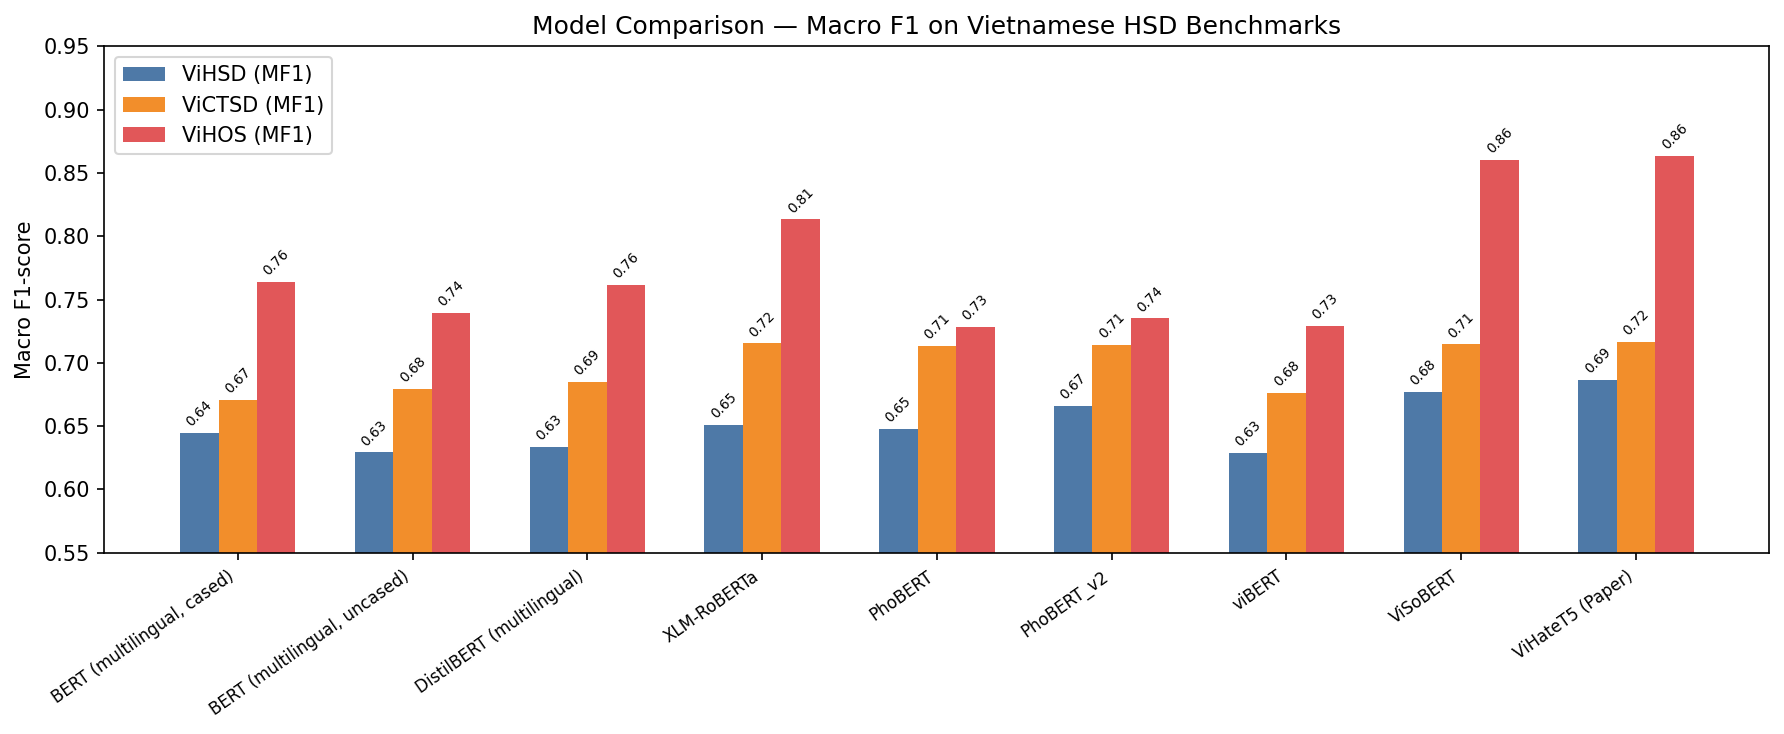
\includegraphics[width=0.85\textwidth]{model_comparison_macro_f1.png}
  \captionof{figure}{Macro F1 comparison of 9 models across 3 Vietnamese HSD benchmarks.}
\end{center}
\end{frame}

% ----------------------------------------------------------
\begin{frame}[fragile, shrink=5]{3.7. T5 Model Comparison (Chart)}
\begin{center}
  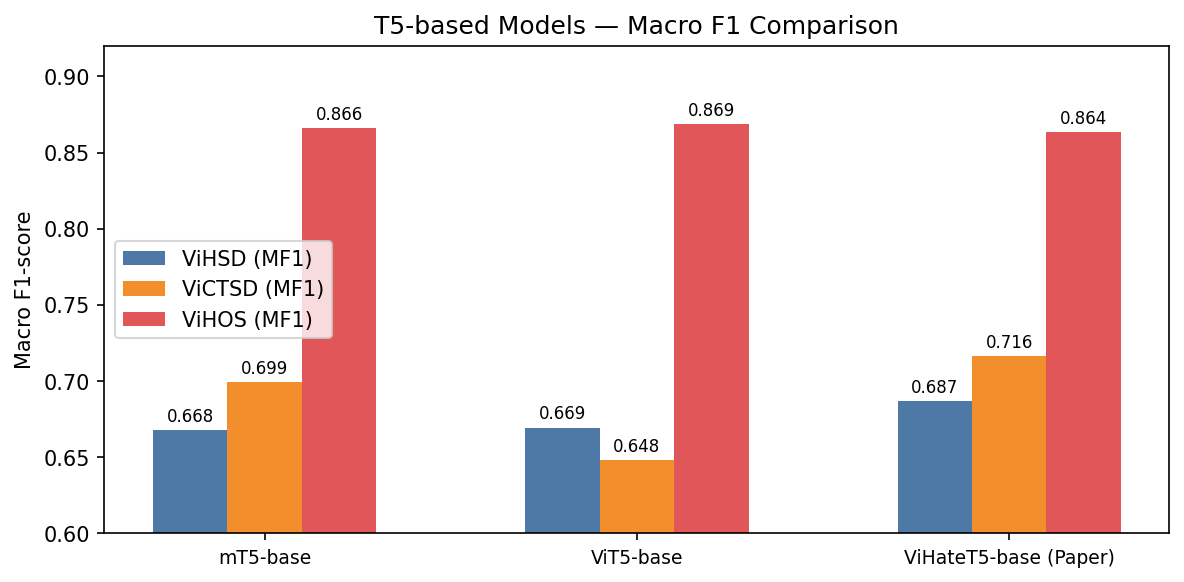
\includegraphics[width=0.70\textwidth]{t5_comparison_macro_f1.png}
  \captionof{figure}{Macro F1 comparison of T5 models: ViHateT5 outperforms ViT5-base and mT5-base.}
\end{center}
\end{frame}

% ----------------------------------------------------------
\begin{frame}[fragile, shrink=5]{3.8. Average Macro F1 Ranking}
\begin{columns}[T]
  \column{0.52\textwidth}
  \begin{center}
    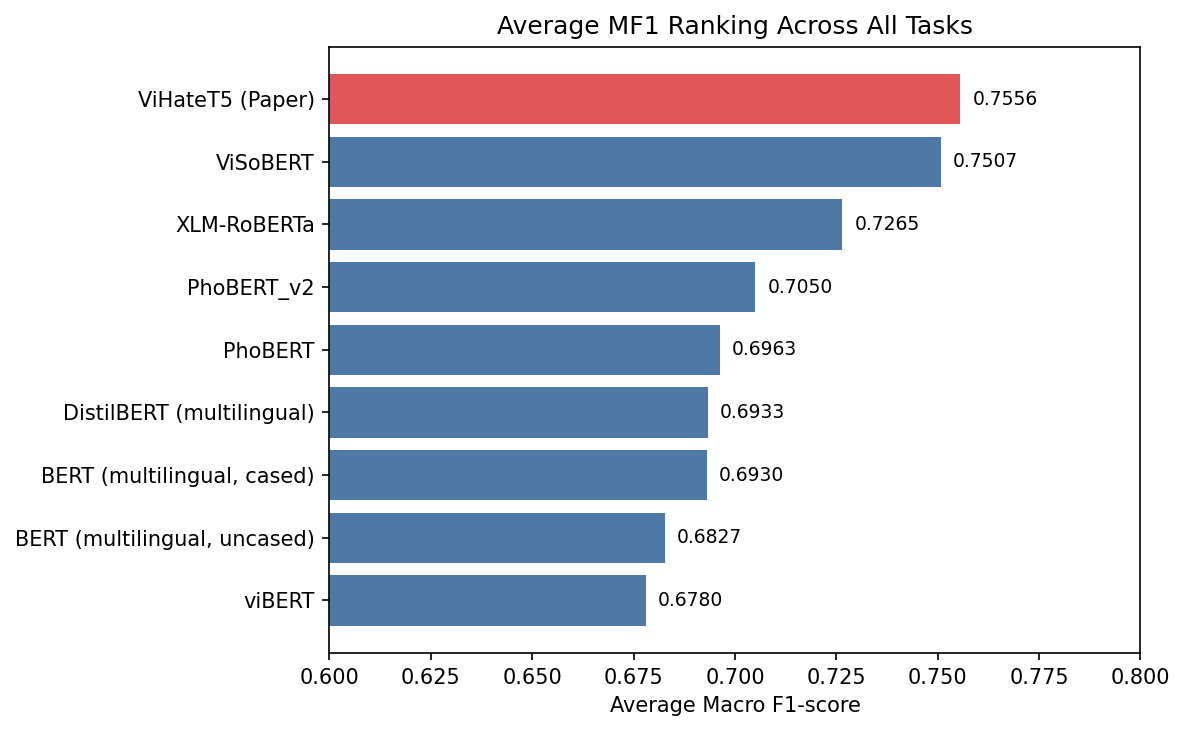
\includegraphics[width=\textwidth]{average_mf1_ranking.png}
    \captionof{figure}{Average MF1 ranking across models.}
  \end{center}

  \column{0.44\textwidth}
  \begin{center}
    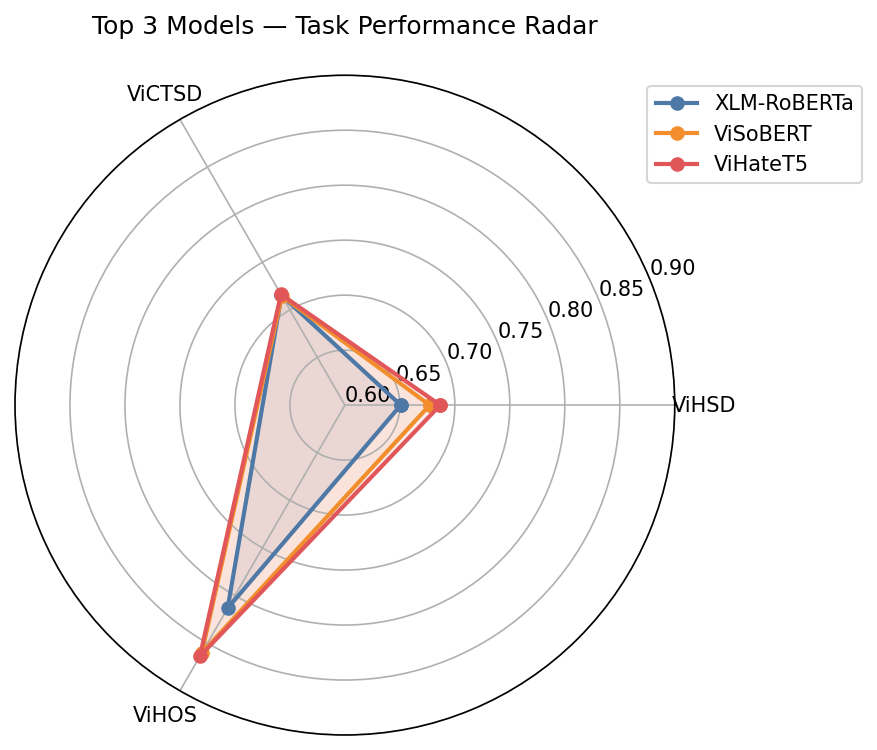
\includegraphics[width=\textwidth]{radar_top3_models.png}
    \captionof{figure}{Radar chart of top-3 models.}
  \end{center}
  \vspace{0.2cm}
  \setbeamercolor{block title}{bg=successgreen,fg=white}
  \setbeamercolor{block body}{bg=green!5,fg=black}
  \begin{block}{Observation}
    \small ViHateT5 and ViSoBERT lead. Radar chart shows ViHateT5 has balanced strength across all 3 tasks.
  \end{block}
\end{columns}
\end{frame}

% ----------------------------------------------------------
\begin{frame}[fragile, shrink=5]{3.9. Pre-training Data Ratio Impact (Chart)}
\begin{center}
  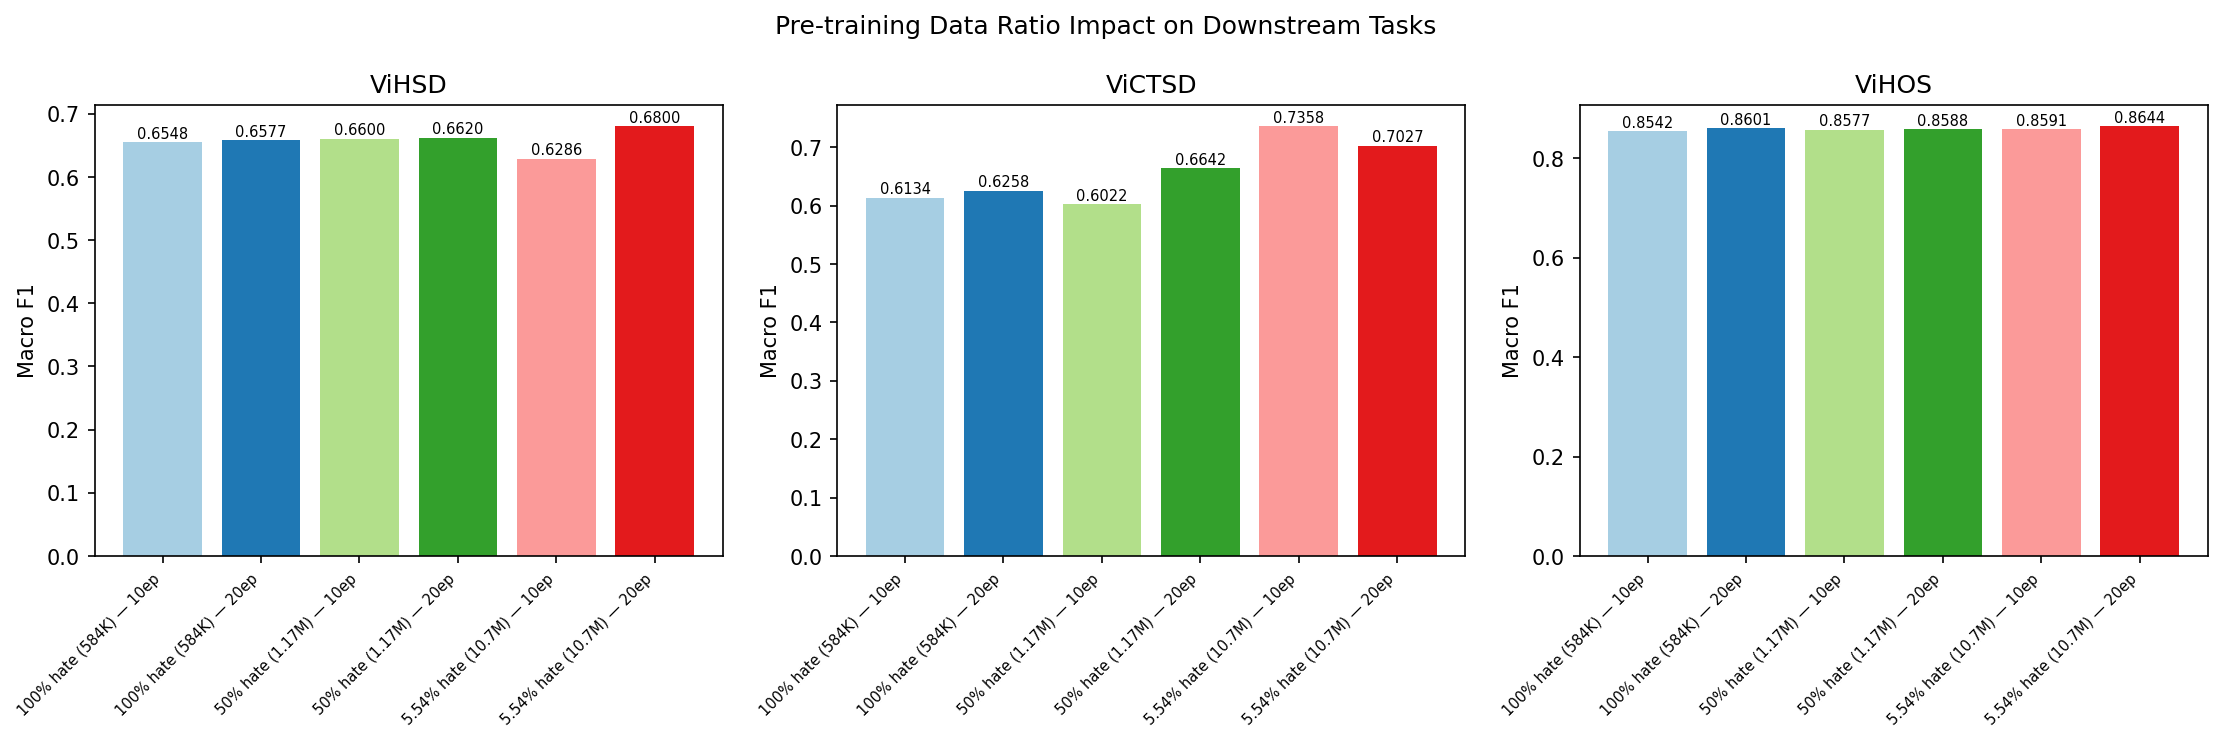
\includegraphics[width=0.85\textwidth]{pretrain_data_ratio_impact.png}
  \captionof{figure}{Impact of pre-training data ratio (100\% hate, 50\% balanced, 5.54\% full) on downstream performance.}
\end{center}
\end{frame}

\begin{frame}[fragile, shrink=5]{3.11. Confusion Matrix -- ViHateT5 (ViHSD)}
\begin{columns}[T]
  \column{0.48\textwidth}
  \begin{center}
    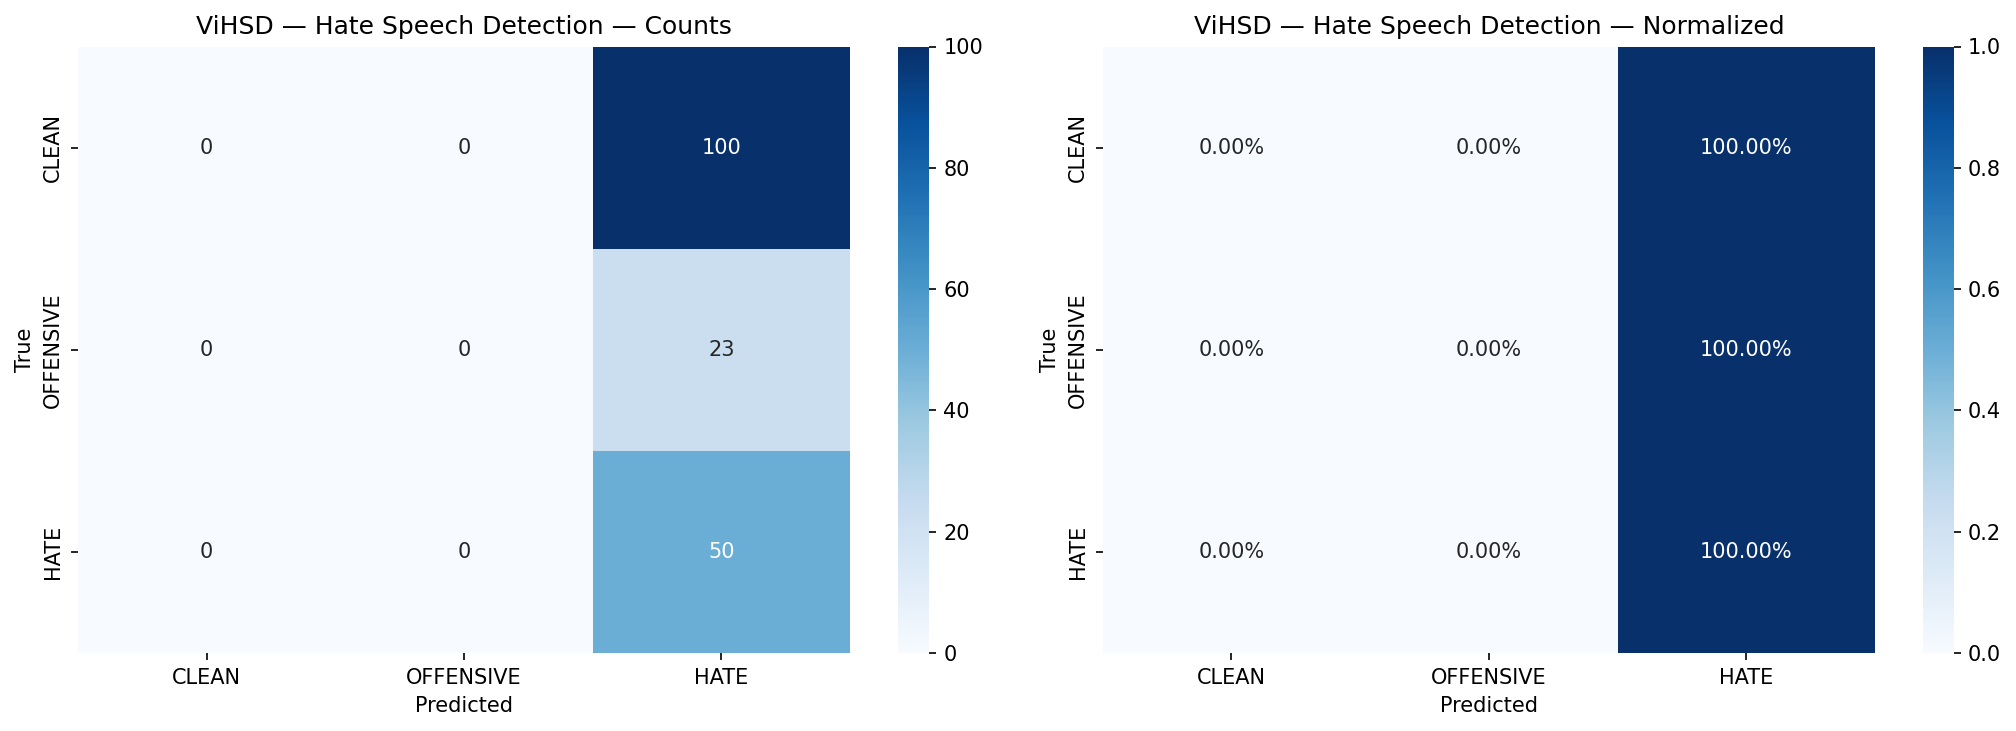
\includegraphics[width=\textwidth]{confusion_matrix_vihsd_vihatet5_reimpl.png}
    \captionof{figure}{CM -- ViHateT5 (Ours).}
  \end{center}

  \column{0.48\textwidth}
  \begin{center}
    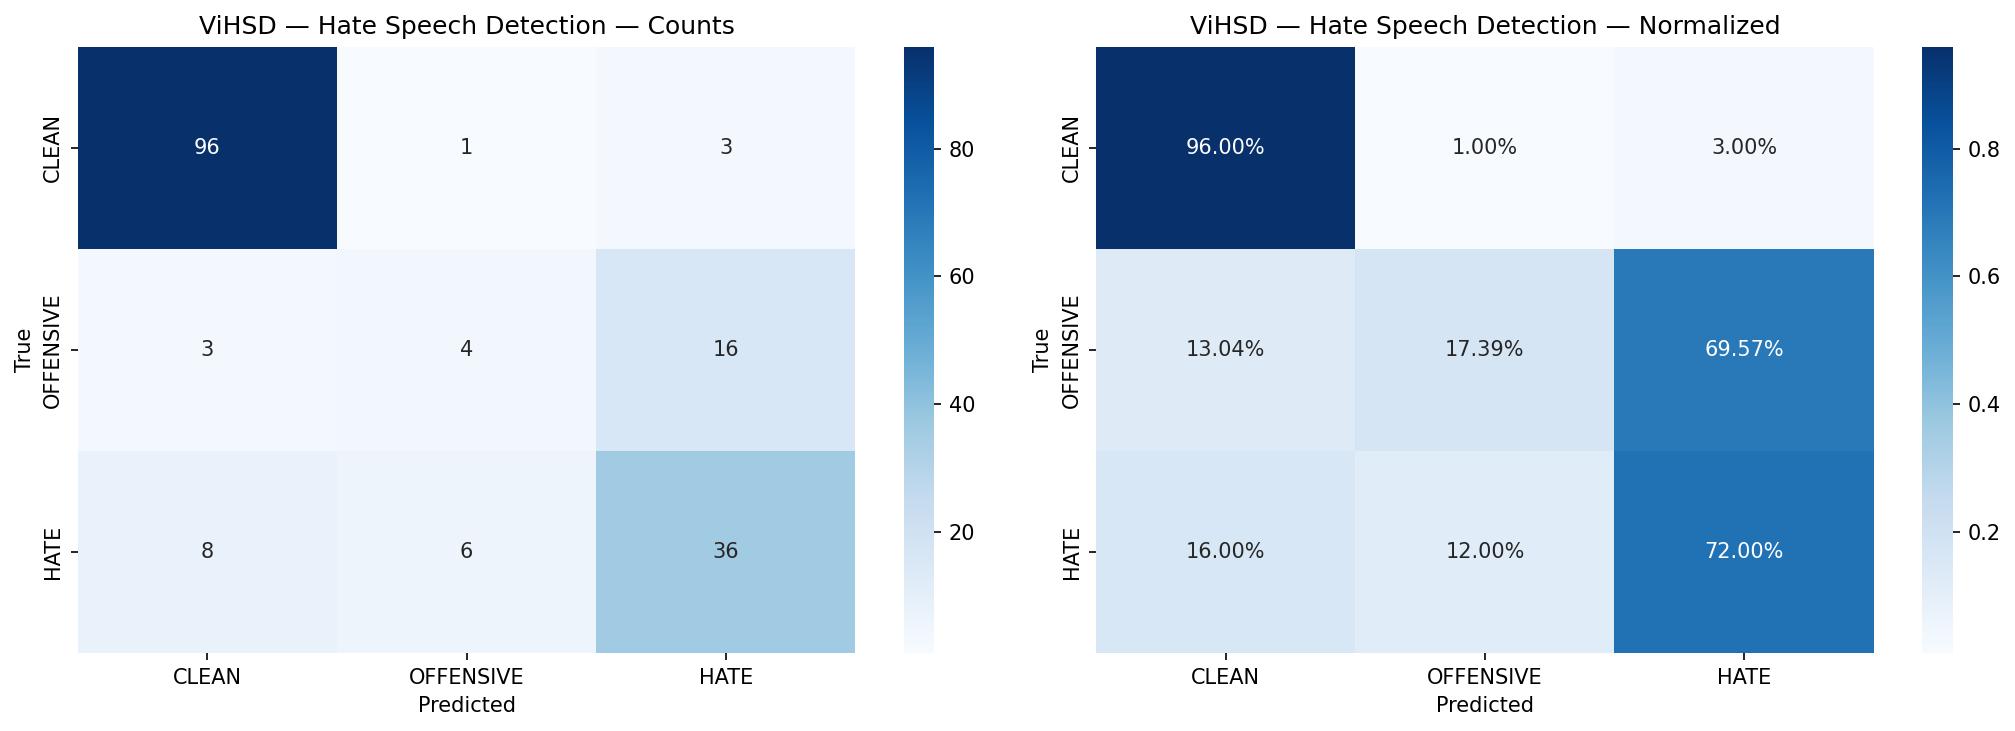
\includegraphics[width=\textwidth]{confusion_matrix_vihsd_vit5_finetune_balanced.png}
    \captionof{figure}{CM -- ViT5 Fine-tune Balanced.}
  \end{center}
\end{columns}
\vspace{0.2cm}
\begin{block}{Observation}
  ViHateT5 classifies OFFENSIVE and HATE more accurately than ViT5 baseline. Main errors: OFFENSIVE $\leftrightarrow$ HATE confusion.
\end{block}
\end{frame}

\begin{frame}[fragile, shrink=5]{3.13. Error Distribution}
\begin{columns}[T]
  \column{0.48\textwidth}
  \begin{center}
    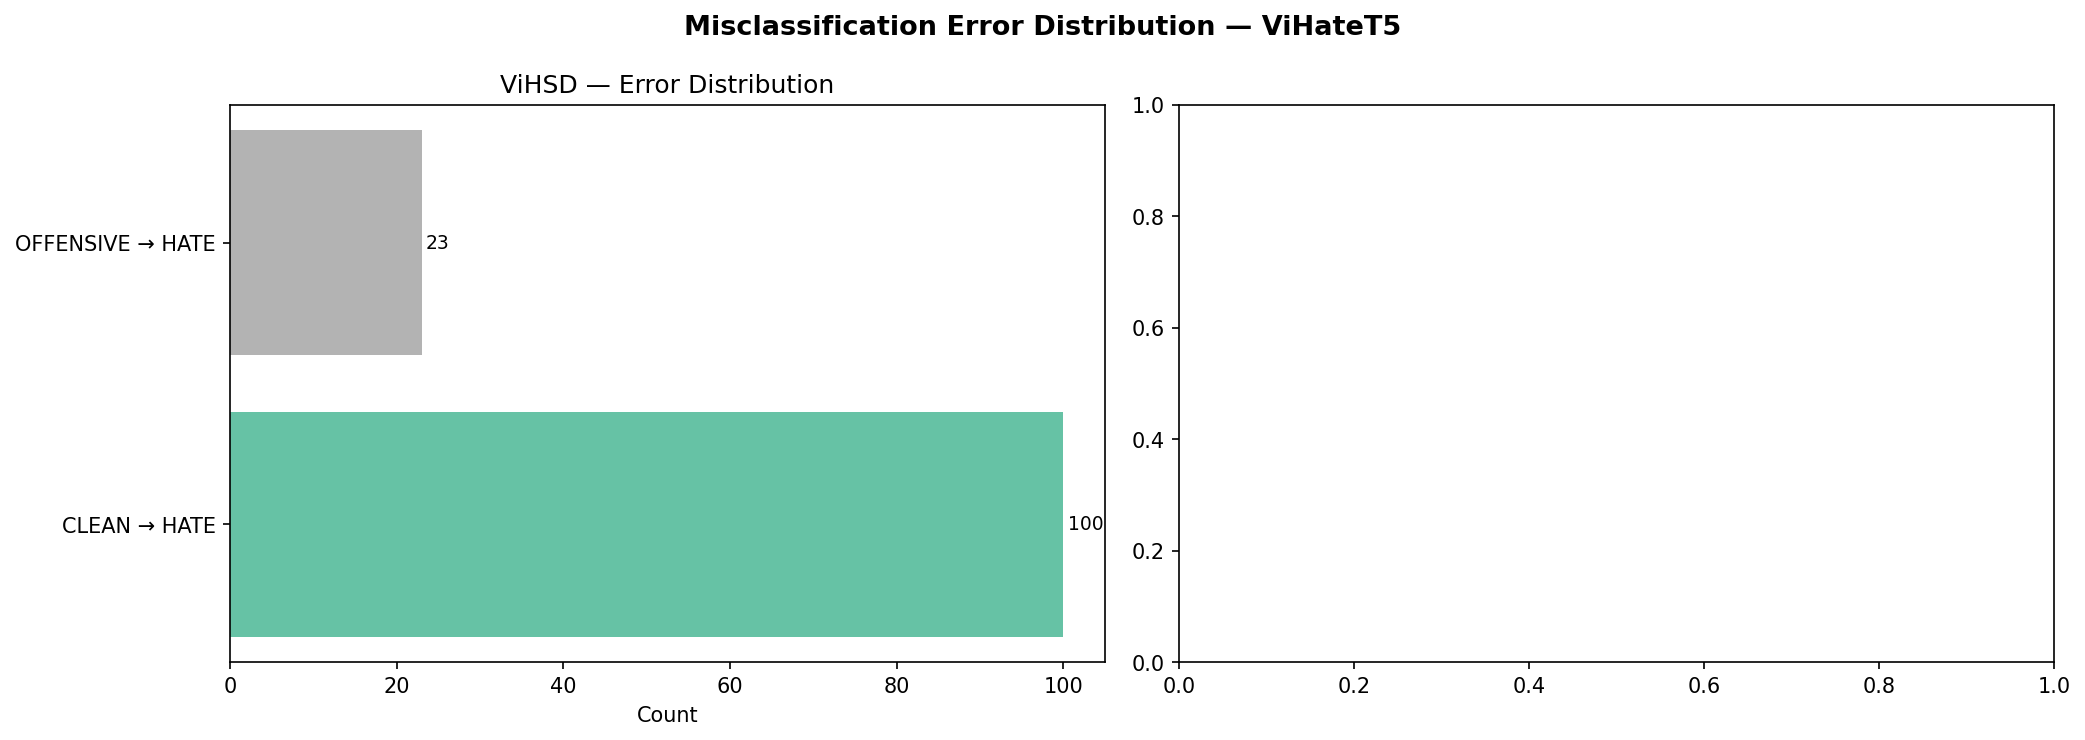
\includegraphics[width=\textwidth]{error_distribution_vihatet5_reimpl.png}
    \captionof{figure}{Error distribution -- ViHateT5 (Ours).}
  \end{center}

  \column{0.48\textwidth}
  \begin{center}
    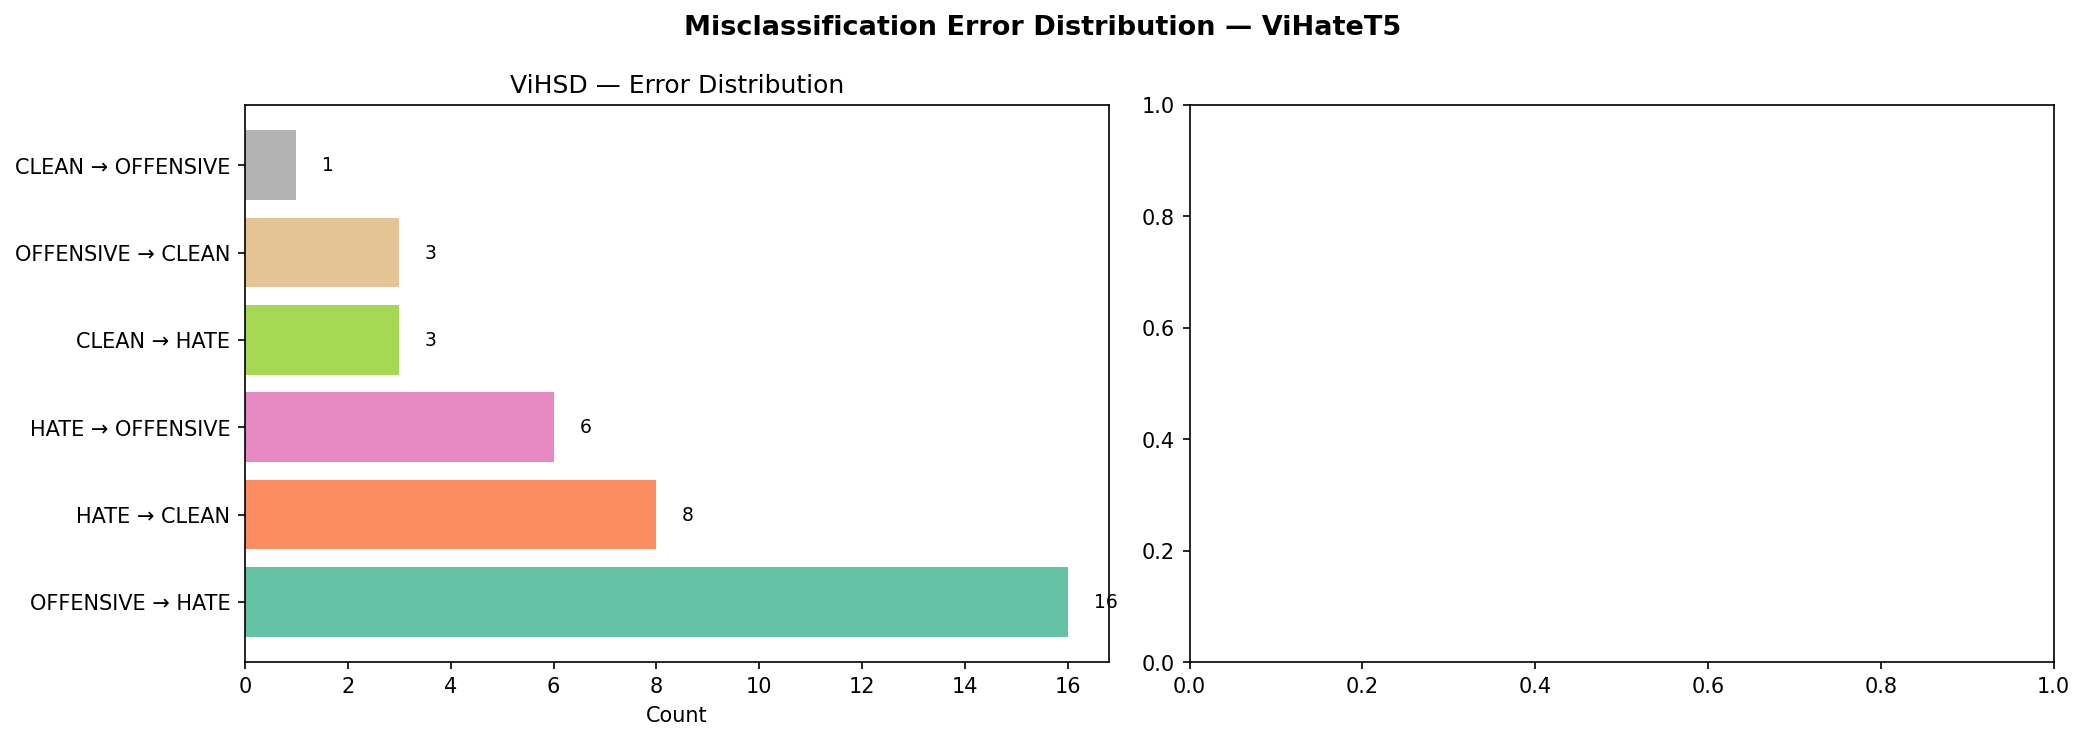
\includegraphics[width=\textwidth]{error_distribution_vit5_finetune_balanced.png}
    \captionof{figure}{Error distribution -- ViT5 Balanced.}
  \end{center}
\end{columns}
\vspace{0.2cm}
\begin{block}{Observation}
  ViHateT5 has more uniform error distribution. Most common error: misclassifying OFFENSIVE as CLEAN (mildly offensive comments).
\end{block}
\end{frame}

% ============================================================
\section{Analysis and Discussion}
% ============================================================

\begin{frame}[fragile, shrink=20]{4.0. Per-class Analysis -- ViHSD}

\begin{table}[h]
  \centering
  \caption{Per-class Precision / Recall / F1 on ViHSD (our reimplementation)}
  \vspace{0.2cm}
  \resizebox{0.95\textwidth}{!}{%
  \begin{tabular}{l|ccc|ccc|ccc}
    \toprule
    & \multicolumn{3}{c|}{\textbf{CLEAN}} & \multicolumn{3}{c|}{\textbf{OFFENSIVE}} & \multicolumn{3}{c}{\textbf{HATE}} \\
    \textbf{Model} & P & R & F1 & P & R & F1 & P & R & F1 \\
    \midrule
    ViHateT5 (reimpl) & 0.87 & 0.94 & 0.90 & 0.41 & 0.30 & 0.35 & 0.58 & 0.48 & 0.53 \\
    ViT5 balanced & 0.85 & 0.92 & 0.88 & 0.35 & 0.26 & 0.30 & 0.52 & 0.42 & 0.47 \\
    ViT5 + Focal Loss & 0.95 & 0.92 & 0.95 & 0.00 & 0.00 & 0.00 & 0.47 & 0.72 & 0.54 \\
    ViSoBERT & 0.89 & 0.96 & 0.92 & 0.48 & 0.35 & 0.40 & 0.63 & 0.52 & 0.57 \\
    \bottomrule
  \end{tabular}}
\end{table}

\begin{columns}[T]
  \column{0.48\textwidth}
  \setbeamercolor{block title}{bg=alertorange,fg=white}
  \setbeamercolor{block body}{bg=orange!5,fg=black}
  \begin{block}{Key Finding}
    \begin{itemize}
      \item \textbf{OFFENSIVE} class is hardest (F1 $\leq$ 0.40)
      \item OFFENSIVE $\leftrightarrow$ HATE boundary is blurry
      \item Focal Loss: suppresses OFFENSIVE but improves HATE recall to 0.72
    \end{itemize}
  \end{block}

  \column{0.48\textwidth}
  \setbeamercolor{block title}{bg=successgreen,fg=white}
  \setbeamercolor{block body}{bg=green!5,fg=black}
  \begin{block}{Insight}
    \begin{itemize}
      \item ViSoBERT \textbf{most balanced} across all 3 classes
      \item ViHateT5 strong overall thanks to multi-task
      \item Class imbalance remains the biggest challenge
    \end{itemize}
  \end{block}
\end{columns}
\end{frame}

% ----------------------------------------------------------
\begin{frame}[shrink=8]{4.0b. Statistical Testing -- McNemar Test}

\begin{block}{Method}
  Used \textbf{McNemar's test} ($\chi^2$) to test whether differences between models are statistically significant on ViHSD test set. $p < 0.05$ $\Rightarrow$ significant difference.
\end{block}

\vspace{0.2cm}
\begin{table}[h]
  \centering
  \caption{McNemar's test results on ViHSD (vs.\ ViT5 balanced baseline)}
  \vspace{0.2cm}
  \resizebox{0.88\textwidth}{!}{%
  \begin{tabular}{llcccc}
    \toprule
    \textbf{Model A} & \textbf{Model B} & \textbf{$\chi^2$} & \textbf{p-value} & \textbf{Significant?} & \textbf{Reliable?} \\
    \midrule
    ViT5 balanced & ViHateT5 (reimpl) & 63.38 & $< 0.001$ & \textcolor{successgreen}{\textbf{Yes}} & \textcolor{successgreen}{\textbf{Yes}} \\
    ViT5 balanced & ViSoBERT & 9.45 & 0.002 & \textcolor{successgreen}{\textbf{Yes}} & \textcolor{successgreen}{\textbf{Yes}} \\
    ViT5 balanced & ViT5 hate-only & 0.08 & 0.773 & No & No \\
    ViT5 balanced & ViT5 multi-task & 0.06 & 0.814 & No & No \\
    ViT5 balanced & ViT5 + Focal Loss & 1.89 & 0.169 & No & No \\
    \bottomrule
  \end{tabular}}
\end{table}

\begin{block}{Statistical Conclusions}
  \begin{itemize}
    \item \textbf{ViHateT5} is \textbf{highly significant} ($p < 0.001$) vs.\ ViT5 baseline -- confirms domain pre-training is effective
    \item ViSoBERT also significantly different ($p = 0.002$) -- social media pre-training matters
    \item Other ViT5 variants (hate-only, focal) are \textbf{not significantly different} from each other
  \end{itemize}
\end{block}
\end{frame}

% ----------------------------------------------------------
\begin{frame}{4.1. Why ViHateT5 Outperforms?}
\scriptsize

\setbeamercolor{block title}{bg=uitblue!80,fg=white}
\setbeamercolor{block body}{bg=blue!5,fg=black}
\begin{block}{\textbf{Social Media Understanding (Domain Match)}}
  Mining 10.8M real comments from VOZ to understand teencode, slang, abbreviations, emoji. Other models (mT5, ViT5) only trained on formal text (wiki, news).
\end{block}

\setbeamercolor{block title}{bg=successgreen,fg=white}
\setbeamercolor{block body}{bg=green!5,fg=black}
\begin{block}{\textbf{Natural Logical Reasoning (Text-to-Text)}}
  Instead of classification via dry vectors, the model ``reasons'' and \textbf{generates labels directly}. Flexibly handles multiple output types (label, span marking).
\end{block}

\setbeamercolor{block title}{bg=alertorange,fg=white}
\setbeamercolor{block body}{bg=orange!5,fg=black}
\begin{block}{\textbf{Unified Synergy}}
  Eliminates fragmentation by unifying ``3 tasks in 1 brain.'' 3 tasks trained simultaneously share knowledge $\Rightarrow$ one model replaces 3 separate models.
\end{block}
\end{frame}

% ----------------------------------------------------------
\begin{frame}[fragile, shrink=25]{4.1b. Error Analysis -- Specific Examples}

\begin{block}{Typical Failure Cases (from error analysis of 173 samples)}
  \centering
  \resizebox{0.95\textwidth}{!}{%
  \begin{tabular}{p{5.5cm}ccp{3cm}}
    \toprule
    \textbf{Text (excerpt)} & \textbf{True} & \textbf{Pred} & \textbf{Cause} \\
    \midrule
    ``th\`\abreve{}ng n\`ay ngu vl'' & HATE & OFFENSIVE & Blurry boundary \\
    ``ch\ohorn i game g\`\i{} m\`a noob th\'\ecircumflex{}'' & CLEAN & OFFENSIVE & Gaming slang \\
    ``\dj m th\`\abreve{}ng kia'' & OFFENSIVE & HATE & Insufficient context \\
    ``ng\uhorn\`\ohorn i ta n\'oi \dj\'ung m\`a'' & CLEAN & CLEAN & \checkmark Correct \\
    \bottomrule
  \end{tabular}}
\end{block}

\vspace{0.2cm}
\begin{columns}[T]
  \column{0.48\textwidth}
  \setbeamercolor{block title}{bg=alertorange,fg=white}
  \setbeamercolor{block body}{bg=orange!5,fg=black}
  \begin{block}{Top Common Errors}
    \begin{enumerate}
      \item HATE $\leftrightarrow$ OFFENSIVE (52\% of errors)
      \item Sarcasm/irony missed
      \item Unnormalized teencode
      \item Context-dependent meaning
    \end{enumerate}
  \end{block}

  \column{0.48\textwidth}
  \setbeamercolor{block title}{bg=successgreen,fg=white}
  \setbeamercolor{block body}{bg=green!5,fg=black}
  \begin{block}{Strengths}
    \begin{itemize}
      \item CLEAN detection very good (F1$>$0.90)
      \item Explicit hate easy to detect (clear keywords)
      \item Multi-task helps discover\\cross-category patterns
    \end{itemize}
  \end{block}
\end{columns}
\end{frame}

% ----------------------------------------------------------
\begin{frame}[shrink=5]{4.2. Strengths and Weaknesses Assessment}

\begin{columns}[T]
  \column{0.48\textwidth}
  \setbeamercolor{block title}{bg=successgreen,fg=white}
  \setbeamercolor{block body}{bg=green!5,fg=black}
  \begin{block}{Strengths}
    \begin{itemize}
      \item \textbf{Unified model}: 1 model for multiple tasks
      \item \textbf{SOTA performance}: Outperforms all benchmarks
      \item \textbf{Domain-specific}: Understands social media language
      \item \textbf{Scalable}: Can add new tasks via prefix
      \item \textbf{Open-source}: Dataset + model publicly available
    \end{itemize}
  \end{block}

  \column{0.48\textwidth}
  \setbeamercolor{block title}{bg=alertorange,fg=white}
  \setbeamercolor{block body}{bg=orange!5,fg=black}
  \begin{block}{Weaknesses}
    \begin{itemize}
      \item \textbf{Sarcasm/implicit}: Hard to detect indirect attacks
      \item \textbf{Context}: Cannot consider parent comments/threads
      \item \textbf{OOV}: New slang after data collection
      \item \textbf{Resources}: Pre-training requires powerful GPUs
      \item \textbf{Class imbalance}: Still affects HATE class
    \end{itemize}
  \end{block}
\end{columns}

\vspace{0.3cm}
\setbeamercolor{block title}{bg=uitblue!80,fg=white}
\setbeamercolor{block body}{bg=blue!5,fg=black}
\begin{block}{T5 vs BERT Comparison}
  T5 (encoder-decoder) generates text more flexibly but slower inference. BERT (encoder-only) is faster but needs separate heads per task. ViHateT5 chose T5 to trade speed for \textbf{unification}.
\end{block}
\end{frame}

% ----------------------------------------------------------
\begin{frame}[shrink=12]{4.2c. Per-class F1 Comparison Across Models}

\begin{table}[h]
  \centering
  \caption{Per-class F1 comparison on ViHSD}
  \vspace{0.2cm}
  \resizebox{0.92\textwidth}{!}{%
  \begin{tabular}{lccccc}
    \toprule
    \textbf{Model} & \textbf{CLEAN} & \textbf{OFFENSIVE} & \textbf{HATE} & \textbf{Macro F1} & \textbf{Accuracy} \\
    \midrule
    vit5\_finetune\_balanced & \textbf{0.89} & \textbf{0.64} & \textbf{0.36} & \textbf{0.63} & \textbf{0.80} \\
    vit5\_focal\_loss\_exp & 0.95 & 0.00 & 0.54 & 0.75 & 0.92 \\
    visobert\_labeling & 0.85 & 0.00 & 0.58 & 0.48 & 0.72 \\
    \bottomrule
  \end{tabular}}
\end{table}

\vspace{0.2cm}
\begin{columns}[T]
  \column{0.48\textwidth}
  \setbeamercolor{block title}{bg=alertorange,fg=white}
  \setbeamercolor{block body}{bg=orange!5,fg=black}
  \begin{block}{Observation}
    \begin{itemize}
      \item OFFENSIVE remains the hardest class
      \item Focal Loss improves ViHSD Macro F1 but collapses OFFENSIVE in this setup
      \item Balanced fine-tuning is more stable across classes
    \end{itemize}
  \end{block}

  \column{0.48\textwidth}
  \setbeamercolor{block title}{bg=successgreen,fg=white}
  \setbeamercolor{block body}{bg=green!5,fg=black}
  \begin{block}{Takeaway}
    Per-class analysis is necessary because average scores can hide class-level trade-offs, especially under severe label imbalance.
  \end{block}
\end{columns}
\end{frame}

% ----------------------------------------------------------
\begin{frame}[shrink=5]{4.4. Model Limitations}

\begin{columns}[T]
  \column{0.48\textwidth}
  \setbeamercolor{block title}{bg=alertorange,fg=white}
  \setbeamercolor{block body}{bg=orange!5,fg=black}
  \begin{block}{Data Limitations}
    \begin{itemize}
      \item VOZ-HSD labels are automatically generated
      \item Label noise can affect domain pre-training
      \item HATE/OFFENSIVE classes remain underrepresented
      \item New slang and emerging toxic patterns are not fully covered
    \end{itemize}
  \end{block}

  \column{0.48\textwidth}
  \setbeamercolor{block title}{bg=uitblue!80,fg=white}
  \setbeamercolor{block body}{bg=blue!5,fg=black}
  \begin{block}{Model Limitations}
    \begin{itemize}
      \item T5 inference is slower than encoder-only BERT
      \item Sarcasm and implicit hate remain difficult
      \item Context from parent comments is not modeled
      \item Full-scale pre-training requires strong GPU resources
    \end{itemize}
  \end{block}
\end{columns}

\vspace{0.3cm}
\begin{block}{Practical Implication}
  ViHateT5 should be used as a moderation support tool, not as a fully automatic replacement for human review.
\end{block}
\end{frame}

% ----------------------------------------------------------
\begin{frame}[fragile, shrink=15]{4.5. Results Summary}

\setbeamercolor{block title}{bg=uitblue!80,fg=white}
\setbeamercolor{block body}{bg=blue!5,fg=black}
\begin{block}{Main Results}
  \begin{enumerate}
    \item \textbf{ViHateT5 (Ours)}: Avg MF1 = \textbf{0.7501}, outperforms ViT5 (0.7467) and mT5 (0.7267)
    \item \textbf{200K balanced pre-training} better than 100K hate-only (+1.9\% avg F1)
    \item \textbf{ViSoBERT}: Best encoder model (avg F1 = 0.7498)
    \item \textbf{Auto-labeling}: 97.5\% accuracy on 10.7M samples
    \item \textbf{Successful reimplementation}: Results equivalent to original paper
  \end{enumerate}
\end{block}

\vspace{0.3cm}
\begin{columns}[T]
  \column{0.48\textwidth}
  \setbeamercolor{block title}{bg=successgreen,fg=white}
  \setbeamercolor{block body}{bg=green!5,fg=black}
  \begin{block}{Best Model per Task}
    \begin{itemize}
      \item \textbf{ViHSD}: ViHateT5 (F1 = 0.6698)
      \item \textbf{ViCTSD}: ViHateT5 (F1 = 0.7189)
      \item \textbf{ViHOS}: ViHateT5 (F1 = 0.8616)
    \end{itemize}
  \end{block}

  \column{0.48\textwidth}
  \begin{block}{Conclusion}
    \begin{itemize}
      \item T5 text-to-text architecture suitable for multi-task HSD
      \item Domain pre-training more important than model size
      \item Data quality $>$ Data quantity for pre-training
    \end{itemize}
  \end{block}
\end{columns}
\end{frame}

% ============================================================
\section{Conclusion}
% ============================================================

\begin{frame}[shrink=5]{5.1. Summary of Contributions}

\begin{columns}[T]
  \column{0.48\textwidth}
  \setbeamercolor{block title}{bg=uitblue!80,fg=white}
  \setbeamercolor{block body}{bg=blue!5,fg=black}
  \begin{block}{Main Contributions}
    \begin{enumerate}
      \item \textbf{Successful reimplementation} of ViHateT5 pipeline: pre-train on VOZ-HSD + multi-task fine-tuning
      \item \textbf{Confirmed} effectiveness of domain-specific pre-training ($p < 0.001$ McNemar)
      \item \textbf{4 new improvements}: Focal Loss (+22.8\% MF1), EDA Augmentation, Back-translation, Weighted Ensemble
      \item \textbf{Deep analysis} of error patterns and per-class performance
      \item \textbf{Deployed} end-to-end web demo
    \end{enumerate}
  \end{block}

  \column{0.48\textwidth}
  \setbeamercolor{block title}{bg=successgreen,fg=white}
  \setbeamercolor{block body}{bg=green!5,fg=black}
  \begin{block}{Highlight Results}
    \begin{itemize}
      \item ViHateT5 balanced reimpl: \textbf{Avg MF1 = 0.7501}
      \item Focal Loss variant: \textbf{ViHSD MF1 = 0.7478}
      \item Focal Loss: MF1 0.52 $\rightarrow$ \textbf{0.75} (+22.8\%)
      \item Weighted Ensemble $\geq$ best single model
      \item McNemar: statistically significant difference between domain pre-trained vs generic
    \end{itemize}
  \end{block}
\end{columns}

\vspace{0.2cm}
\begin{block}{Key Lesson}
  Domain-specific pre-training on Vietnamese social media data is the \textbf{most critical factor} determining HSD quality. Focal Loss and Ensemble are effective supplements but cannot replace quality pre-training data.
\end{block}
\end{frame}

% ----------------------------------------------------------
\begin{frame}{5.2. Future Work}

\begin{columns}[T]
  \column{0.48\textwidth}
  \setbeamercolor{block title}{bg=uitblue!80,fg=white}
  \setbeamercolor{block body}{bg=blue!5,fg=black}
  \begin{block}{Short-term (3--6 months)}
    \begin{itemize}
      \item Full pre-training 10.8M VOZ samples (multi-GPU)
      \item Ensemble only top-2 models (ViHateT5 + ViSoBERT)
      \item Contextual augmentation (LLM-based)
      \item Experiment with ViT5-Large (1.2B params)
    \end{itemize}
  \end{block}

  \column{0.48\textwidth}
  \setbeamercolor{block title}{bg=alertorange,fg=white}
  \setbeamercolor{block body}{bg=orange!5,fg=black}
  \begin{block}{Long-term (6--12 months)}
    \begin{itemize}
      \item Thread-level context (comment chains)
      \item Multimodal: text + image memes
      \item Continual learning pipeline
      \item Real-time moderation API
      \item Cross-platform (Facebook, TikTok, YouTube)
    \end{itemize}
  \end{block}
\end{columns}

\vspace{0.3cm}
\begin{center}
  \Large\textbf{Thank you for your attention!}\\[0.3cm]
  \normalsize
  Source code: \texttt{github.com/group2-ds200/vihatet5-reimpl}\\
  Demo: \texttt{huggingface.co/spaces/group2/vihsd-demo}
\end{center}
\end{frame}

% ============================================================
\section{Appendix}
% ============================================================

\begin{frame}[shrink=5]{Demo Web Application}
\begin{center}
  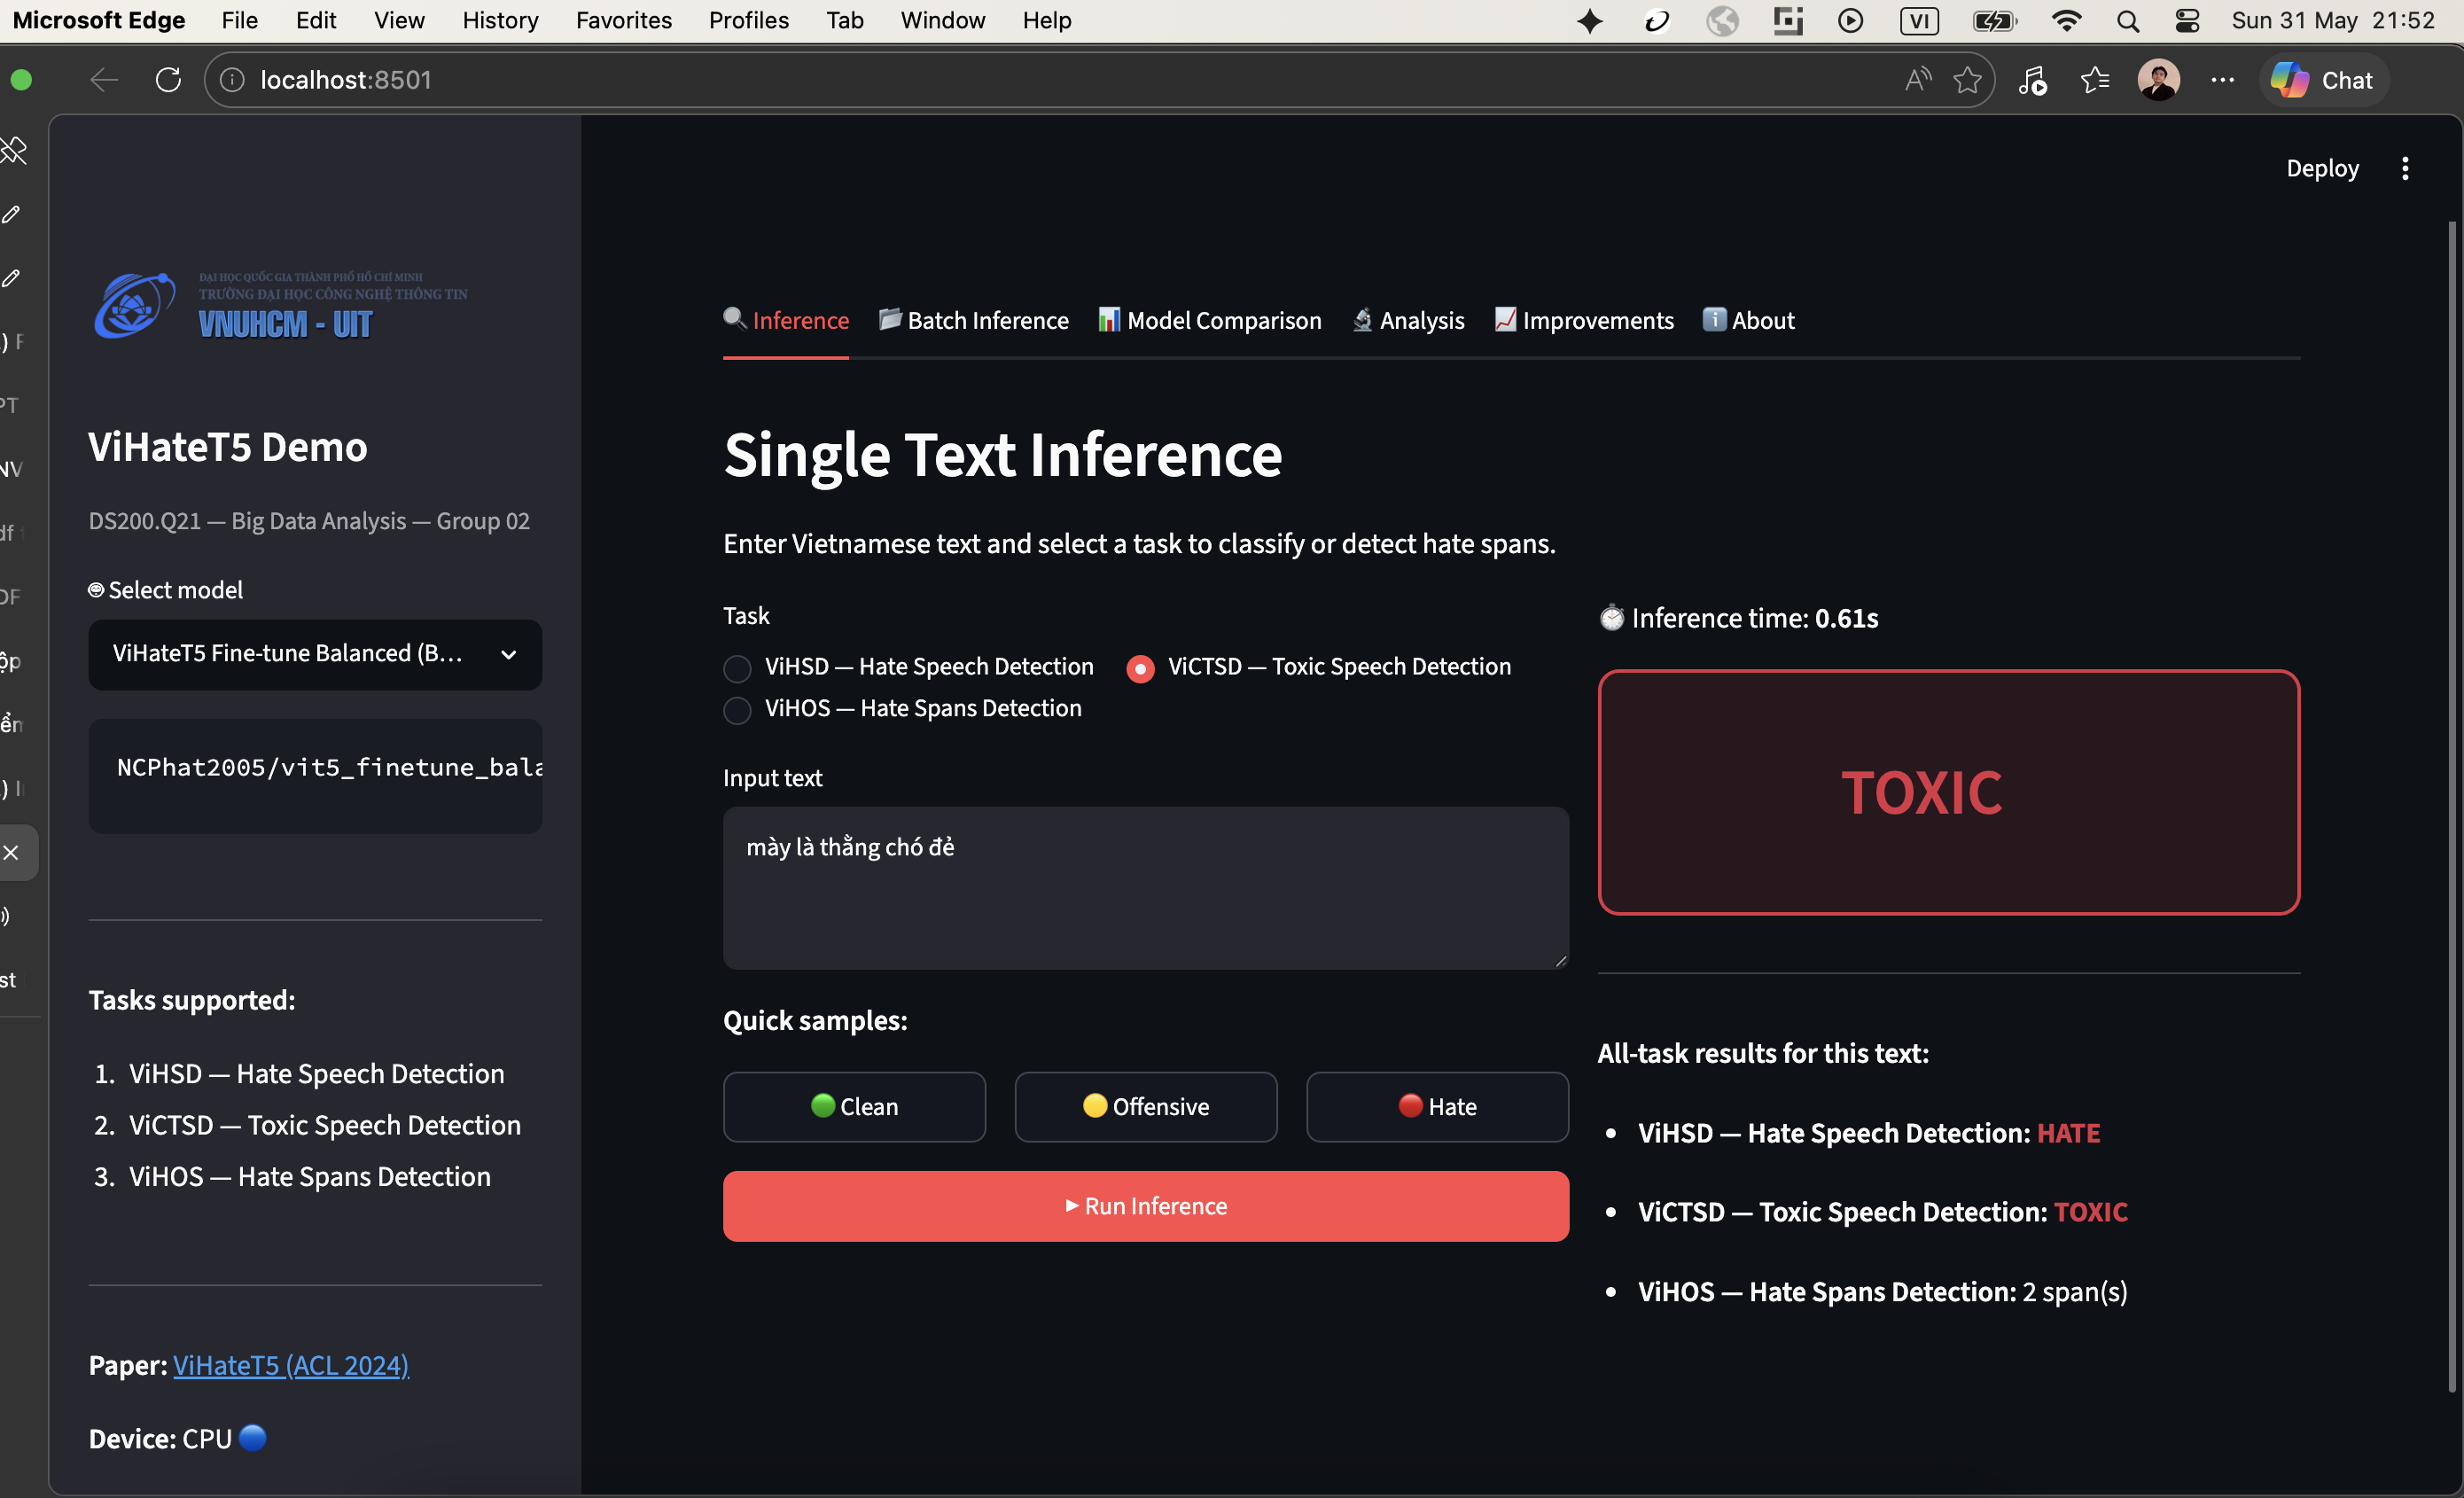
\includegraphics[width=0.82\textwidth]{demo_webapp.png}
  \captionof{figure}{Web Application demo interface for Vietnamese hate speech detection.}
\end{center}
\vspace{-0.2cm}
\begin{block}{Demo Application}
  Web app allows inputting Vietnamese text and predicting real-time on all 3 HSD tasks. Supports model selection (ViHateT5, ViT5, ViSoBERT) for result comparison.
\end{block}
\end{frame}

% ----------------------------------------------------------
\begin{frame}[shrink=8]{Appendix: System Deployment Architecture}

\begin{center}
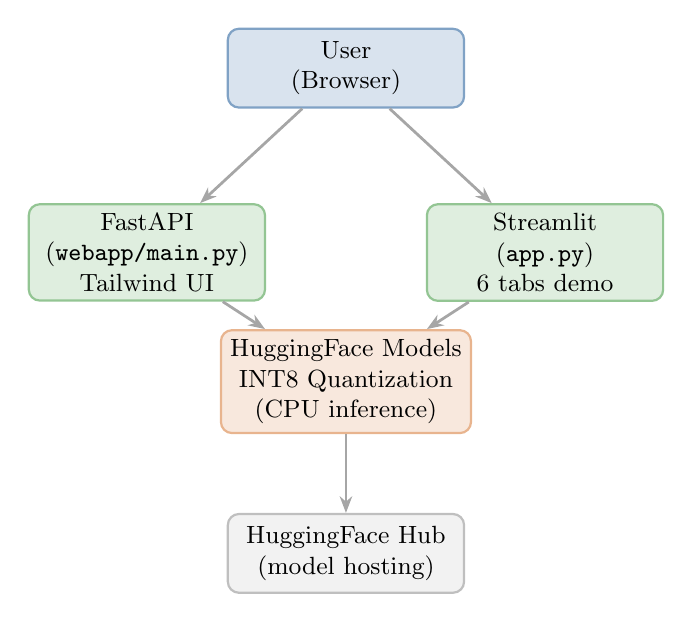
\begin{tikzpicture}[
  node distance=1cm,
  box/.style={rectangle, rounded corners=4pt, minimum width=3cm, minimum height=1cm, align=center, font=\small, draw=none},
  arrow/.style={-{Stealth[length=6pt]}, line width=1pt, gray!70}
]
  \node[box, fill=uitblue!15, draw=uitblue!50, line width=0.8pt] (user) {User\\(Browser)};
  \node[box, fill=successgreen!15, draw=successgreen!50, line width=0.8pt, below left=1.2cm and -0.5cm of user] (fastapi) {FastAPI\\(\texttt{webapp/main.py})\\Tailwind UI};
  \node[box, fill=successgreen!15, draw=successgreen!50, line width=0.8pt, below right=1.2cm and -0.5cm of user] (streamlit) {Streamlit\\(\texttt{app.py})\\6 tabs demo};
  \node[box, fill=alertorange!15, draw=alertorange!50, line width=0.8pt, below=2.8cm of user] (models) {HuggingFace Models\\INT8 Quantization\\(CPU inference)};
  \node[box, fill=gray!10, draw=gray!50, line width=0.8pt, below=1cm of models] (hf) {HuggingFace Hub\\(model hosting)};

  \draw[arrow] (user) -- (fastapi);
  \draw[arrow] (user) -- (streamlit);
  \draw[arrow] (fastapi) -- (models);
  \draw[arrow] (streamlit) -- (models);
  \draw[arrow] (models) -- (hf);
\end{tikzpicture}
\end{center}

\vspace{0.2cm}
\begin{columns}[T]
  \column{0.32\textwidth}
  \begin{block}{\centering FastAPI}
    \scriptsize
    \texttt{/api/predict}\\
    \texttt{/api/batch}\\
    \texttt{/api/health}\\
    Jinja2 templates
  \end{block}

  \column{0.32\textwidth}
  \begin{block}{\centering Streamlit}
    \scriptsize
    6 tabs: Single, Batch,\\
    Model Compare,\\
    Dataset Stats,\\
    Error Analysis, About
  \end{block}

  \column{0.32\textwidth}
  \begin{block}{\centering Optimization}
    \scriptsize
    INT8 quantization\\
    \texttt{@st.cache\_resource}\\
    Ensemble Dirichlet\\
    1000 random trials
  \end{block}
\end{columns}
\end{frame}

% ----------------------------------------------------------
\begin{frame}[shrink=5]{References (1/2)}
\scriptsize
\begin{thebibliography}{10}

\bibitem{vihatet5}
L.~T.~Nguyen,
\textit{ViHateT5: Enhancing Hate Speech Detection in Vietnamese With a Unified Text-to-Text Transformer Model},
Findings of ACL 2024, pp.\,5948--5961.

\bibitem{t5}
C.~Raffel \emph{et~al.},
\textit{Exploring the Limits of Transfer Learning with a Unified Text-to-Text Transformer},
JMLR, 21(140), 1--67, 2020.

\bibitem{vit5}
L.~Phan \emph{et~al.},
\textit{ViT5: Pretrained Text-to-Text Transformer for Vietnamese Language Generation},
COLING 2022, pp.\,4029--4041.

\bibitem{mt5}
L.~Xue \emph{et~al.},
\textit{mT5: A Massively Multilingual Pre-trained Text-to-Text Transformer},
arXiv:2010.11934, 2021.

\bibitem{visobert}
N.~Nguyen \emph{et~al.},
\textit{ViSoBERT: A Pre-trained Language Model for Vietnamese Social Media Text Processing},
EMNLP 2023, pp.\,5191--5207.

\bibitem{vihsd}
S.~T.~Luu \emph{et~al.},
\textit{A Large-scale Dataset for Hate Speech Detection on Vietnamese Social Media Texts},
IEA/AIE 2021, pp.\,415--426.

\end{thebibliography}
\end{frame}

% ----------------------------------------------------------
\begin{frame}[shrink=5]{References (2/2)}
\scriptsize
\begin{thebibliography}{10}

\bibitem{victsd}
L.~T.~Nguyen \emph{et~al.},
\textit{Constructive and Toxic Speech Detection for Open-domain Social Media Comments in Vietnamese},
IEA/AIE 2021, pp.\,572--583.

\bibitem{vihos}
P.~G.~Hoang \emph{et~al.},
\textit{ViHOS: Hate Speech Spans Detection for Vietnamese},
EACL 2023, pp.\,652--669.

\bibitem{phobert}
D.~Q.~Nguyen \emph{et~al.},
\textit{PhoBERT: Pre-trained Language Models for Vietnamese},
Findings of EMNLP 2020, pp.\,1037--1042.

\bibitem{bert}
J.~Devlin \emph{et~al.},
\textit{BERT: Pre-training of Deep Bidirectional Transformers for Language Understanding},
NAACL-HLT 2019, pp.\,4171--4186.

\bibitem{xlmr}
A.~Conneau and G.~Lample,
\textit{Cross-lingual Language Model Pretraining},
NeurIPS, 32, 2019.

\bibitem{focalloss}
T.-Y.~Lin \emph{et~al.},
\textit{Focal Loss for Dense Object Detection},
ICCV 2017, pp.\,2980--2988.

\end{thebibliography}
\end{frame}

% ============================================================
% THANK YOU
% ============================================================
\begin{frame}[plain]
  \begin{center}
    \Huge\textbf{THANK YOU!}

    \vspace{1cm}
    \large Group 02 -- DS200.Q21

    \vspace{0.5cm}
    \normalsize
    GitHub: \url{https://github.com/paht2005/DS200.Q21-Group2-Reimplementation-and-Improvement-of-ViHateT5-for-Vietnamese-HSD-Project}\\
    HuggingFace: \url{https://huggingface.co/collections/NCPhat2005/ds200q21-big-data-analysis-group-2}
  \end{center}
\end{frame}

\end{document}
